\chapter{Correlation based penalty function}\label{chap:rpr}

In this chapter, we propose a novel regularization factor to penalize the use of features highly correlated with a protected attribute by a machine learning model, aiming to avoid the redlining effect~\citep{Pedreschi2008}. The proposed penalization factor is applied directly to the input weights of a Multi-Layer Perceptron, using a strategy that proportionately penalizes features use based on their correlation with the sensitive feature.

\section{Preliminaries} \label{sec:rpr_preliminaries}

The phenomena known as redlining effect~\citep{Pedreschi2008} consists in the unintended use of proxy variables to the sensitive feature by the model, which can lead model to produce indirect discrimination in their outcomes.  Thus, the insight here is to penalize the use of those proxy features by the model proportionally according its correlation with sensitive feature in order to avoid redlining effed. The proposed regularization approach uses the recently described Chatterjee's xi correlation coefficient~\cite{chatterjee2020new}, which robustly asses whether a random variable can be described as a function of another one, as a measure of the potential of given feature to be used by the model as a proxy to the sensitive feature. 

Before discussing this approach, we start defining some common correlation coefficients and providing a proper comparison within Chatterjee's correlation. For purpose of simplicity we describe only the most commonly used form, more complex formulations involving additional terms depending on available data should be considered to most of coefficients. Also, we present some related approaches, specially those ones that, like ours, use regularization and penalty factors to avoid indirect discrimination.

The Pearson correlation coefficient, denoted by $\rho$ and defined in Definition~\ref{def:pearson}, is a measure of the linear relationship between two random variables. The Pearson correlation coefficient ranges from $-1$ to $1$, where $1$ indicates a perfect positive linear relationship, $-1$ indicates a perfect negative linear relationship, and $0$ indicates no linear relationship.

\begin{definition}[Pearson correlation coefficient]\label{def:pearson}
Let  $X$ and $Y$\ random variables. The Pearson correlation coefficient $\rho$ between $X$ and $Y$ can be defined as  
\begin{equation}
\rho = \frac{\mathrm{Cov}(X, Y)}{\sigma_X \sigma_Y},
\end{equation}
where $\mathrm{Cov}(X, Y)$ is the covariance between $X$ and $Y$, while $\sigma_X$ and $\sigma_Y$ the standard deviations of $X$ and $Y$, respectively. 
\end{definition}

Spearman's rank correlation coefficient, denoted by $\rho_s$ and defined in Definition~\ref{def:spearman}, measures the strength and direction of the monotonic relationship between two ranked (ordered) variables.  As like Pearson correlation coefficient, Spearman's rank correlation coefficient ranges from $-1$ to $1$, where $1$ indicates a perfect positive relationship, $-1$ indicates a perfect negative relationship, and $0$ indicates no relationship.
 
\begin{definition}[Spearman's correlation coefficient]\label{def:spearman}
Let $X$ and $Y$\ random variables, $n$ the sample size and $X_i, \, Y_i$ the $i$-th observations to $i = 1 \ldots n$. Let $R_{X_i}, \, R_{Y_i}$ the rank of observations $X_i, \, Y_i$, i.e. the position of $X_i, \, Y_i$ by ordering the samples, respectively. The Spearman's rank correlation coefficient  $\rho_s$ between $X$ and $Y$ can be defined to non-repeated observation values as 
\begin{equation}\label{eq:spearman}
\rho_s = 1 - \frac{6 \sum\limits_{i=1}^{n}d_i^2}{n(n^2 - 1)},
\end{equation}
where $d_i = R_{X_i} - R_{Y_i}$.
\end{definition}

Kendall's rank correlation coefficient, denoted by $\tau$ and defined in Definition~\ref{def:kendall},  indicates the strength and direction of association between two variables. It is based on the relative ordering of pairs of observations rather than their actual values. Here we interpret the correlation values as like in Spearman's and Pearson's correlation coefficients, ranging from $-1$ to $1$, where $1$ indicates a perfect positive relationship, $-1$ a perfect negative relationship, and $0$  no linear relationship.

\begin{definition}[Kendall's correlation coefficient]\label{def:kendall}
Let two variables $X$ and $Y$ sampled with $n$ pairs of observations $(X_i, Y_i)$ for $i = 1, 2, \ldots, n$. A pair of observations $(X_i, Y_i)$ and $(X_j, Y_j)$ is \textbf{concordant} if the ranks (order) of both elements agree, i.e., to $i < j$ either $X_i > X_j$ and $Y_i > Y_j)$ or $X_i < X_j$ and $Y_i < Y_j$. Otherwise their are considered \textbf{discordant}, i.e., either $X_i > X_j$ and $Y_i < Y_j$ or $X_i < X_j$ and $Y_i > Y_j$. The Kendall's rank correlation coefficient $\tau$ between $X$ and $Y$ can be defined as 
\begin{equation}\label{eq:kendall}
\tau = \frac{2(N_c - N_d)}{n(n-1)},
\end{equation}
where $N_c$ is the number of concordant observation and $N_d$ the number of discordant observations.
\end{definition}

Chatterjee's rank correlation coefficient, denoted by $\xi$ and defined in Definition~\ref{def:chatterjee}, is designed to robustly measure the degree of dependence between two variables without assuming any specific type of relationship and capturing noise nuances.  The previously described correlation coefficients are not effective on detecting associations that are not monotonic, even in complete absence of noise.

This correlation coefficient asses whether a random variable can be described as a function of another one. Differently from correlation coefficients described before, this coefficient ranges from 0 to 1, where 0 indicates independence and 1 indicates a perfect functional relationship. Also this correlation is not symmetric, i.e., the correlation between $X$ and $Y$ may differ from between $Y$ and $X$. 

\begin{definition}[Chatterjee's correlation coefficient]\label{def:chatterjee}
Let two variables $X$ and $Y$ , where $Y$ is not a constant, sampled with $n$ pairs of observations $(X_i, Y_i)$ for $i = 1, 2, \ldots, n$. The Chatterjee's rank correlation coefficient $\tau$ between $X$ and $Y$ when there are no ties among $Y$ can be defined as 
\begin{equation}\label{eq:chatterjee}
\xi = 1 - \frac{3 \sum\limits_{i=1}^{n-1} |R_{i+1} - R_i|}{n^2 - 1},
\end{equation}
where $R_i$ is the rank of $Y_i$ in the ordered sequence of $Y$ values corresponding to the sorted $X$ values. 
\end{definition}

To illustrate some characteristics of Chatterjee's rank correlation coefficient we compare those results on Anscombe's quartet~\citep{anscombe1973} along with Pearson's, Spearman's and Kendall's correlation coefficients. The Anscombe's quartet (Table~\ref{tab:anscombe}) is a set of four different datasets that have nearly identical simple descriptive statistics, yet very different distribution, which is clear on Figure~\ref{fig:anscombe}. As an additional resource, a line representing a linear regression over the data is plotted within the points, enforcing that they present nearly identical simple descriptive statistics.

\begin{table}[ht]
\centering
\caption{Anscombe's quartet}
\label{tab:anscombe}
\begin{tabular}{rr|rr|rr|rr}
\toprule
\multicolumn{2}{c|}{I} & \multicolumn{2}{c|}{II} & \multicolumn{2}{c|}{III} & \multicolumn{2}{c}{IV} \\

\multicolumn{1}{c}{$x$} & \multicolumn{1}{c|}{$y$} & \multicolumn{1}{c}{$x$} & \multicolumn{1}{c|}{$y$} & \multicolumn{1}{c}{$x$} & \multicolumn{1}{c|}{$y$} & \multicolumn{1}{c}{$x$} & \multicolumn{1}{c}{$y$} \\
\midrule
10.0 & 8.04 & 10.0 & 9.14 & 10.0 & 7.46 & 8.0 & 6.58 \\
8.0 & 6.95 & 8.0 & 8.14 & 8.0 & 6.77 & 8.0 & 5.76 \\
13.0 & 7.58 & 13.0 & 8.74 & 13.0 & 12.74 & 8.0 & 7.71 \\
9.0 & 8.81 & 9.0 & 8.77 & 9.0 & 7.11 & 8.0 & 8.84 \\
11.0 & 8.33 & 11.0 & 9.26 & 11.0 & 7.81 & 8.0 & 8.47 \\
14.0 & 9.96 & 14.0 & 8.10 & 14.0 & 8.84 & 8.0 & 7.04 \\
6.0 & 7.24 & 6.0 & 6.13 & 6.0 & 6.08 & 8.0 & 5.25 \\
4.0 & 4.26 & 4.0 & 3.10 & 4.0 & 5.39 & 19.0 & 12.50 \\
12.0 & 10.84 & 12.0 & 9.13 & 12.0 & 8.15 & 8.0 & 5.56 \\
7.0 & 4.82 & 7.0 & 7.26 & 7.0 & 6.42 & 8.0 & 7.91 \\
5.0 & 5.68 & 5.0 & 4.74 & 5.0 & 5.73 & 8.0 & 6.89 \\
\bottomrule
\end{tabular}
\end{table}

Comparing correlation coefficients, it is evident that Pearson's $\rho$ does not properly capture the peculiarities of Anscombe's quartet. Although the four datasets present the same correlation coefficient, they exhibit very different distribution. Spearman's $\rho_s$ and Kendall's $\tau$ performs very similarly each other, properly capturing relevant characteristics, albeit Kendall's $\tau$ demonstrates to be more exigent on assigning high correlation values. Chatterjee's $\xi$ is even more exigent, pursuing the behavior of capturing functional relations between data, considering noise. For example, the first quartet presents a small $\xi$ as it contains relevant noise, despite the points are effectively linearly disposed. Albeit the second quartet demonstrate a non linear distribution, the data has lower noise influence, presenting a more functional relationship. Thus, to Chatterjee's correlation the second presents a higher coefficient than the first, which is not equivalently captured by Spearman's and Kendall's. 
\begin{figure}[!ht]
\centering
\caption{Multiple correlation coefficients on Anscombe's quartet.}\label{fig:anscombe}
    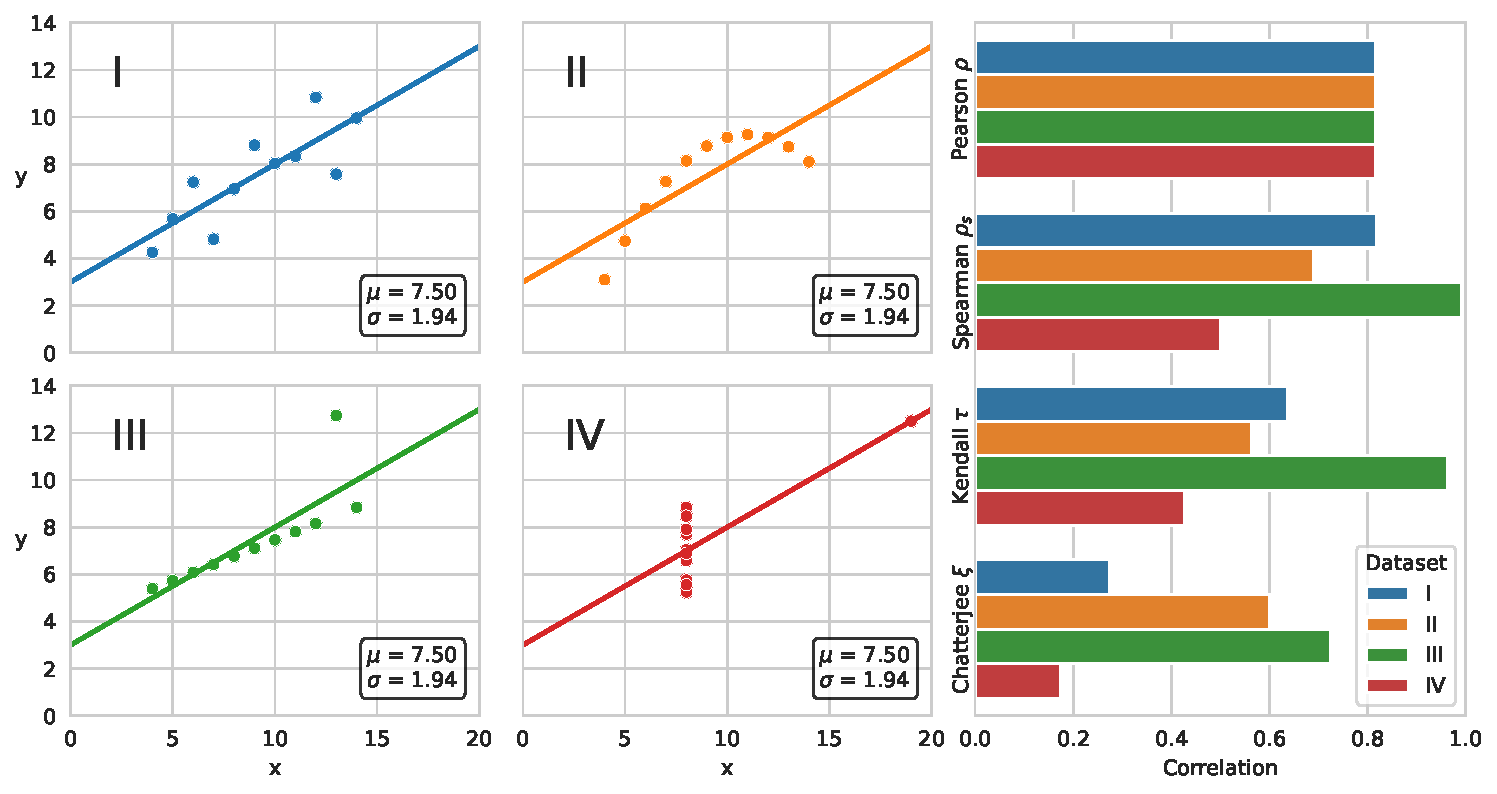
\includegraphics[width=1\linewidth]{images/anscombe_quartet.pdf}
\end{figure}



As a resource to defining the proposed redlining penalty method we describe the L2 regularization. This regularization term, a.k.a. weight decay, is a common technique used to prevent overfitting in machine learning models, including the Multi-Layer Perceptron (MLP). The L2 regularization adds a penalty term to the loss function that is proportional to the sum of the squares of the model parameters (weights). This encourages the model to keep the weights small, which can help improving generalization.

Let $\mathbf{W}^{(l)}$ represent the weight matrix for the $l$-th layer of the MLP, and let $\mathbf{b}^{(l)}$ denote the corresponding bias vector. The primary loss function of the network, $L_0$, could be any suitable loss function such as the mean squared error for regression or the cross-entropy loss for classification. The L2 regularization term for a single layer is given by
\begin{equation}
R(\mathbf{W}^{(l)}) = \frac{1}{2} \sum_{i=1}^{d_l} \sum_{j=1}^{h_l} \left( W^{(l)}_{ij} \right)^2,
\end{equation}
where $d_l$ and $h_l$ are the dimensions of the weight matrix $\mathbf{W}^{(l)}$, and $W^{(l)}_{ij}$ is the weight connecting the $i$-th input neuron to the $j$-th neuron in the $l$-th layer. Thus, the total regularization term for the entire network, considering all layers, is
\begin{equation}
R(\mathbf{W}) = \frac{1}{2} \sum_{l=1}^{L} \sum_{i=1}^{d_l} \sum_{j=1}^{h_l} \left( W^{(l)}_{ij} \right)^2,
\end{equation}
where $L$ is the total number of layers in the network. Furthermore, the total loss function $L$ for the MLP, incorporating the L2 regularization term, is defined as
\begin{equation}
L = L_0 + \lambda \; R(\mathbf{W}),
\end{equation}
where $\lambda$ is a scalar hyperparameter that controls the overall strength of the regularization.

By adding this regularization term, the optimization process aims to minimize the primary loss $L_0$ along with keeping the weights small, thereby helping to reduce the model complexity and prevent overfitting. The gradient descent updates for the weights will be adjusted to account for the regularization term, effectively shrinking the weights during the training process.

Although many fair machine learning techniques are based on imposing constraints to achieve reasonable values under specific fairness definitions and metrics~\citep{Mehrabi2019,caton2023,Hort2023}, the approach of integrating these constraints as regularization factors remains underexplored. One foundational fairness technique, the Prejudice Remover Regularizer~\citep{Kamishima2012}, accomplishes this objective by measuring and penalizing indirect prejudice through a \textit{prejudice index} alongside an L2 regularization.

Relevant regularization approaches to fair machine learning include the dual form for Fairness Constraints through Decision Boundary Covariance by \cite{Zafar2017b} and the example-based and model-agnostic Paired-Consistency approach~\citep{Horesh2020}. A notable approach proposed by \cite{Baharlouei2020} includes a general min-max framework for fair inference using the Rényi correlation coefficient~\citep{Renyi1959} as a regularization term. Additional recent developments in this research area can be found in the works of \cite{Olfat2020}, \cite{Yu2022}, and \cite{jung2023}.

\section{Redlining Penalty Regularizer} \label{sec:rpr_proposal}

Here we propose the Redlining Penalty Regularizer (RPR), a novel regularization term that penalizes the weights of features highly correlated with the sensitive attribute in order to prevent the redlining effect. By incorporating this penalty into the loss function of the neural network, the model is encouraged to reduce its reliance on sensitive attributes and their proxies, thus promoting fairer predictions. To the best of our knowledge, this the first approach to incorporate a regularization term that proportionately penalizes the features weights on the input layer according its correlation to sensitive attribute to prevent the redlining effect.

As referred before, the Chatterjee's Xi Correlation Coefficient distinguish from many other by providing a measure of how much one random variable can be expressed as a function of another, with a range from $0$ to $1$. This characteristics is relevant to the proposed use, to capture redlining effect, as of this phenomena happens exactly when the sensitive feature can be inferred by another one, producing the same harmful effects whether the correlation is positive or negative. Naturally it would be possible to use the absolute value of correlation coefficient such as Pearson, Spearman and Kendall, but this strategy could lead to some kind of information loss. Another relevant characteristics of this correlation coefficient is the ability to capture sophisticated non-linearities, including non-monotonic ones, and the effects of noise on variable's distribution, conditions frequently present in proxy feature relationships. 

Thus, let $X \in \mathbb{R}^{n \times d}$ be a dataset where $n$ represents the number of instances and $d$ represents the number of features. Let $X_i \in \mathbb{R}^n$ denote the $i$-th feature of the dataset, and let $A = X_i \in \mathbb{R}^n$ be a sensitive (protected) feature for some $i$. In this neural network, $\mathbf{W}^{(1)} \in \mathbb{R}^{d \times h}$ is the weight matrix for the first hidden layer, with $h$ being the number of neurons in this layer. Additionally, $\lambda$ is a scalar that controls the overall strength of the regularization.

Thus, the proposed regularization term $R(\mathbf{W}^{(1)})$ applied to the weight matrix $\mathbf{W}^{(1)}$ only on the first hidden layer, defined as 
\begin{equation}\label{eq:xi_reg}
R(\mathbf{W}^{(1)}) = \sum_{i=1}^d \xi_n(X_i,\,A) \sum_{j=1}^h (W^{(1)}_{ij})^2,
\end{equation}
where $W^{(1)}_{ij}$ are the weights connecting the $i$-th input feature to the $j$-th neuron in the first hidden layer. Here, the Chatterjee's Xi Correlation Coefficient $\xi_n(X_i,\,A)$ between the $i$-th input feature $X_i$ and the sensitive feature $A$ acts as the regularization strength for the $i$-th input feature. The greater $i$-th input feature dependence on sensitive feature the greater the penalization factor enforcing lower values to those weights.

Thus, the total loss function $L$ to a MLP, incorporating the sensitive-feature-specific $L_2$ regularization, is defined as
\begin{equation}\label{eq:total_regularized_loss}
L = L_0 + \lambda \; R(\mathbf{W}^{(1)}),
\end{equation}
where $L_0$ is the primary loss function of the network. This formulation ensures that the model's learning process penalizes weights with high values associated with features highly correlated to the sensitive attribute, thereby reducing the potential for biased decisions influenced by redlining effect.

This formulation differs from similar approaches to regularization in order to achieve fairness in machine learning by two fundamental points.  The first one is that here the regularization acts as a focused penalty factor through the use of the correlation of each feature to the sensitive one, reducing it's effect on less correlated features and boosting on the highly correlated ones. The second point is that this proposed penalty does not acts as a common regularizer, by imposing small values on every model's parameter. Rather, it penalizes the use of each feature according it's correlation to the sensitive one by exclusively acting on the input layer weights, that is, the usage level of each feature by hidden units.

With the combination of characteristics tailored by this formulation and the chosen correlation coefficient we do expects effectively avoiding the use of indirect sensitive feature predictors within the model, thus mitigating redlining effect.

\section{Experimental setup} \label{sec:rpr_experimental}

In this section, we detail the experimental setup employed to benchmark the proposed regularization within both Standard MLP with Cross Entropy Loss and a MLP using Fair Transition Loss. Both MLP model uses two hidden layers with $100$ hidden units each, $ReLU$ activation function, batch size of $64$, $50$ epochs early stopped at $3$ epochs without improvement~\citep{Li2020} and softmax in output, trained with ADAM optimizer~\citep{KingmaB14} and learning rate at $3\mathrm{e}{-4}$. 

The overall experimental methodology follows same principles of those used on Fair Transition Loss evaluation. There are two phases: hyperparameter tuning and testing. In the hyperparameter tuning phase we perform a Bandit-Based pruning approach using HyperBand~\citep{Li2018} with Tree-structured Parzen Estimator Sampler (TPE)~\citep{bergstra2011} over $100$ trials. At each trial a fitness function is evaluated by performing a complete training and validation, where both model performance and fairness metrics are assessed. The fitness function is computed based on the objective defined in Equation~\ref{eq:obj_fn}. 

Once the best hyperparameters are selected, we proceed to the testing phase, where a new training is conducted using those optimal hyperparameters. After this training, we evaluate the model's performance on a separate test set that was not used during the hyperparameter tuning phase, which are reported. This complete tuning-training-testing described is repeated $15$ times within random re-sampling then we proceed to comparison. Here the re-sampling consists in shuffling the whole dataset before splitting, as described before

As the objective defined in Equation~\ref{eq:obj_fn} can be achieved with different performance and fairness metrics, we compare the proposed regularization schema within Standard MLP and MLP with FTL in different optimization scenarios, considering as performance metrics Accuracy (Acc.) and Mathews Correlation Coefficient (MCC), while the fairness metrics considered are Statistical Parity (Stat. Parity), Equal Opportunity (Eq. Opp.) and Equalized Odds (Eq. Odds). Those pursued metrics lead us to the following optimization scenarios: MCC and Statistical Parity; MCC and Equal Opportunity; MCC and Equalized Odds; Accuracy and Statistical Parity; Accuracy and Equal Opportunity; Accuracy and Equalized Odds.

\begin{table}[ht]
\centering
\caption{Hyperparameters search ranges or options of each method.}\label{tab:hyperparameters_rpr}
{\footnotesize
\begin{tabular}{lll}
\toprule
Method & Parameter & Range/options \\ \midrule
 Standard MLP without regularization (baseline) & dropout & $[0.0,\,0.2]$  \vspace{1ex} \\
 Standard MLP with RPR & dropout & $[0.0,\,0.2]$  \vspace{1ex} \\
 & $\lambda$ & $\{1e^{-2}, 1^{e-3}, 1^{e-4}\}$ \\
 Fair Transition Loss without regularization & $d_0,p_0,d_1,p_1$ & $[0.0,\,1.0]$ \\
 &  dropout & $[0.0,\,0.2]$ \\
 Fair Transition Loss with RPR & $d_0,p_0,d_1,p_1$ & $[0.0,\,1.0]$ \\
 &  dropout & $[0.0,\,0.2]$ \\
 & $\lambda$ & $\{1e^{-2}, 1^{e-3}, 1^{e-4}\}$ \\
\bottomrule
\end{tabular}
}
\end{table}

Table~\ref{tab:hyperparameters_rpr} presents the methods hyperparameters along with their corresponding search ranges or options. While each method may possess a varying number of hyperparameters and range sizes, all are optimized under the same conditions and number of configurations to guarantee a balanced comparison.

To properly compare this set of $15$ results of each method, we conduct an Almost Stochastic Order (ASO) test \citep{dror2019deep}, a significance test suitable for comparing complex machine learning models with various hyperparameters. As described before, the ASO test involves evaluating a set of metrics through multiple samplings of a Collection of Statistics (in this case assessed in test phase using random resampling) to compare one method against another. The $ASO(A, B)$ function yields a value in the range $[0, 1]$, given two methods $A$ and $B$. If $ASO(A, B)$ is lesser than $0.5$, we can reject the null hypothesis and conclude that method $A$ outperforms method $B$ in the given task. That is, method $A$ produces stochastically larger values than method $B$ for a given metric. The lower the $ASO(A, B)$ value, the stronger the evidence that $A$ is superior to $B$ in that particular task, which can be interpreted as a confidence interval. Therefore, we perform comparisons between all methods for each optimization scenario outlined previously and for each dataset.

Our experiments uses common datasets from Fair Classification benchmarks, namely \textit{Adult Income}~\citep{misc_adult_2}, \textit{German Credit}~\citep{misc_statlog_(german_credit_data)_144}, \textit{Bank Marketing}~\citep{misc_bank_marketing_222}, and \textit{COMPAS Recidivism}~\citep{misc_compas}. We use the dataset readers available in the AI Fairness 360 toolkit~\citep{aif360-oct-2018} with its standard configurations. Instances with missing data are removed. To a proper description of those datasets please check Section~\ref{sec:ftl_experimental}

For all datasets, the data preparation process is the same, one-hot encoding for categorical features and standardize the numerical features. We perform a random split, with $80\%$ allocated for the hyperparameter tuning phase and the remaining $20\%$ reserved for evaluating metrics in the test phase. Within the hyperparameter tuning phase, this corresponding fraction of data is further randomly split, with $80\%$ assigned to training and $20\%$ to validation. The validation set allows us to assess metrics and compute the fitness function for each hyperparameter configuration. In datasets where there is originally some kind of split (e.g., train set and test set in separate files), all available data is merged and then shuffled to produce new splits at each run.

\section{Results and discussion} \label{sec:rpr_results}

Before presenting the main experimental results, we perform an additional comparison using the same methodology to address two concerns. Firstly, one might argue that the proposed penalty strategy does not differs from applying conventional regularization factors like L2. In this context, any observed advantages of the proposed method over the same model without the penalty would be attributed to the conventional effects of regularization, i.e. avoiding model overfitting and consequently improving fitness values. Therefore, we compare the proposed strategy not only with an MLP baseline but also with the same MLP under standard L2 regularization across all network layers, optimized using the ranges specified in Table~\ref{tab:hyperparameters_rpr}.

Secondly, there is the question of whether using traditional correlation coefficients in order to assessing and penalizing redlining , such as Pearson's $\rho$, Spearman's $\rho_s$, and Kendall's $\tau$, would be equally beneficial. To address this, we compare the proposed penalty (referred as RPR$_\xi$) with variations that use the absolute values of Pearson's $\rho$, Spearman's $\rho_s$, and Kendall's $\tau$ instead of Chatterjee's $\xi$, therefore referred as RPR$\rho$, RPR${\rho_s}$, and RPR$\tau$, respectively. In this comparison, every method uses the same MLP architecture and the same hyperparameter tuning procedure, varying only the regularization strategy.

\begin{table}[ht]
    \centering
    \caption{Almost Stochastic Order test comparing RPR$_\xi$ fitness to baseline and multiple regularization schemes. Values under $0.5$ (in bold) mean that RPR$_\xi$ outperforms corresponding method in such optimization scenario.} \label{tab:aso_compare_rpr_variations}
    {\footnotesize
    \begin{tabular}{llccccc}
    \toprule
     \multirow{2}{*}{\shortstack[l]{Fairness/Performance\\Metric}} & Dataset & \multirow{2}{*}{\shortstack[c]{MLP\\(baseline)}} & \multirow{2}{*}{\shortstack[l]{MLP\\L2}} & \multirow{2}{*}{\shortstack[l]{MLP\\RPR$_{\rho}$}} & \multirow{2}{*}{\shortstack[l]{MLP\\RPR$_{\rho_s}$}} & \multirow{2}{*}{\shortstack[l]{MLP\\RPR$_{\tau}$}} \\ \\
\multirow{4}{*}{\shortstack[l]{Statistical Parity\\MCC}} 
 & Adult Income & 0.80 & 0.68 & 1.00 & 0.61 & 0.65 \\
 & Bank Marketing & 1.00 & \textbf{0.46} & 0.80 & 0.74 & 0.59 \\
 & COMPAS Recidivism & \textbf{0.02} & \textbf{0.17} & \textbf{0.18} & \textbf{0.15} & \textbf{0.09} \\
 & German Credit & 1.00 & 1.00 & 1.00 & \textbf{0.24} & 1.00 \\
\midrule
\multirow{4}{*}{\shortstack[l]{Equal Opportunity\\MCC}} 
 & Adult Income & \textbf{0.09} & \textbf{0.03} & \textbf{0.26} & \textbf{0.46} & \textbf{0.28} \\
 & Bank Marketing & 1.00 & 1.00 & 0.79 & 1.00 & 0.55 \\
 & COMPAS Recidivism & \textbf{0.19} & \textbf{0.23} & 0.60 & \textbf{0.33} & 0.89 \\
 & German Credit & 1.00 & 0.71 & 1.00 & 0.89 & 1.00 \\
\midrule
\multirow{4}{*}{\shortstack[l]{Equalized Odds\\MCC}} 
 & Adult Income & \textbf{0.29} & \textbf{0.24} & \textbf{0.25} & 0.63 & \textbf{0.46} \\
 & Bank Marketing & 1.00 & 1.00 & 1.00 & 1.00 & 1.00 \\
 & COMPAS Recidivism & \textbf{0.01} & \textbf{0.04} & \textbf{0.16} & \textbf{0.15} & \textbf{0.01} \\
 & German Credit & 1.00 & 0.63 & \textbf{0.38} & 1.00 & 1.00 \\
\midrule
\multirow{4}{*}{\shortstack[l]{Statistical Parity\\Accuracy}} 
 & Adult Income & 0.76 & \textbf{0.36} & \textbf{0.31} & \textbf{0.47} & \textbf{0.40} \\
 & Bank Marketing & 1.00 & 1.00 & 1.00 & 1.00 & 1.00 \\
 & COMPAS Recidivism & \textbf{0.42} & 0.60 & \textbf{0.48} & 1.00 & 0.72 \\
 & German Credit & 0.92 & 1.00 & 1.00 & 1.00 & 1.00 \\
\midrule
\multirow{4}{*}{\shortstack[l]{Equal Opportunity\\Accuracy}} 
 & Adult Income & \textbf{0.35} & \textbf{0.34} & \textbf{0.26} & 1.00 & \textbf{0.15} \\
 & Bank Marketing & 1.00 & 0.56 & 0.84 & 1.00 & 0.66 \\
 & COMPAS Recidivism & \textbf{0.02} & \textbf{0.04} & \textbf{0.06} & \textbf{0.10} & \textbf{0.19} \\
 & German Credit & 0.65 & 1.00 & 1.00 & 1.00 & 1.00 \\
\midrule
\multirow{4}{*}{\shortstack[l]{Equalized Odds\\Accuracy}} 
 & Adult Income & 1.00 & 0.74 & 0.68 & 0.53 & 0.66 \\
 & Bank Marketing & \textbf{0.19} & \textbf{0.15} & \textbf{0.21} & 0.52 & 0.55 \\
 & COMPAS Recidivism & \textbf{0.09} & \textbf{0.41} & \textbf{0.26} & \textbf{0.36} & \textbf{0.13} \\
 & German Credit & \textbf{0.26} & \textbf{0.11} & \textbf{0.50} & \textbf{0.25} & 1.00 \\
\bottomrule
\end{tabular}
    }
\end{table}

As we have multiple optimization scenarios within different objective functions and datasets, and to each of them multiple runs, we present in Table~\ref{tab:aso_compare_rpr_variations} the results of the ASO test described before, which allow us to properly compare each regularization strategy to RPR$_{\xi}$. Values under $0.5$ (in bold) mean that we can reject the null hypothesis, i.e., RPR$_{\xi}$ produces stochastically larger fitness values than the regularization strategy in respective column for a objective and dataset. Lower values indicate stronger evidence. Additionally, complete results will be available at the end of this section, similar to those presented to the Fair Transition Loss experiments.

Notably, both baseline MLP and MLP with L2 regularization are compatible when juxtaposed to RPR$_{\xi}$ on almost every scenario, i.e. they presents comparable values on ASO test. Both standard MLP and MLP with L2 regularization underperforms when compared to RPR$_{\xi}$. This observation lead us to a comprehension that the proposed penalty schema effectively differs from standard regularization strategies such as L2. Another relevant perception is that the proposed method is highly influenced by the dataset, which will be furthermore explored on this section.

Now we compare the results of the proposed penalty schema using standard correlation coefficients. We can perceive that in almost every scenario where RPR$_{\xi}$ outperforms baseline MLP and MLP with L2 regularization, it also outperforms the same penalty strategy but using standard correlation coefficients instead of Chatterjee's. This enforces the argument that the proposed approach takes advantages of the Chatterjee's correlation coefficient characteristics. Despite that observation, in most of scenarios the ASO values are higher to those produced by baseline MLP and MLP with L2 regularization, indicating that they presents better performance/fairness trade-off. This can be interpret as an ability of the proposed regularization schema to penalizing redlining effect, although less efficiently than when using Chatterjee's correlation coefficient.

\begin{table}[ht]
\centering
\caption{Almost Stochastic Order test comparing the use of Redlining Penalty Regularizer on Standard MLP and MLP with Fair Transition Loss fitness. Values under $0.5$ (in bold) mean that the model with RPR outperforms the same model without regularization on each optimization scenario.} \label{tab:aso_compare_rpr}
{\footnotesize
\begin{tabular}{lrrrr|rrrr}
\toprule
\multirow{2}{*}{Fitness Rule} & \multicolumn{4}{c}{MLP} & \multicolumn{4}{c}{FTL} \\
& Adult & Bank & COMPAS & German & Adult & Bank & COMPAS & German \\
\midrule
MCC - S. Parity & 0.79 & 0.99 & \textbf{0.03} & 1.00 & \textbf{0.34} & 1.00 & 1.00 & \textbf{0.31} \\
MCC - Eq. Opp. & \textbf{0.26} & 1.00 & \textbf{0.01} & 1.00 & \textbf{0.35} & 1.00 & \textbf{0.19} & 1.00 \\
MCC - Eq. Odds & \textbf{0.08} & 1.00 & \textbf{0.20} & 1.00 & \textbf{0.30} & 1.00 & 0.56 & 1.00 \\
Acc. - S. Parity & 0.75 & 1.00 & \textbf{0.39} & 0.87 & \textbf{0.44} & 1.00 & \textbf{0.02} & 1.00 \\
Acc. - Eq. Opp. & 1.00 & \textbf{0.18} & \textbf{0.07} & \textbf{0.24} & 0.58 & 0.67 & 1.00 & 1.00 \\
Acc. - Eq. Odds & \textbf{0.33} & 1.00 & \textbf{0.01} & 0.62 & \textbf{0.40} & 1.00 & \textbf{0.20} & 1.00 \\
\bottomrule
\end{tabular}
}
\end{table}


\begin{figure}[!ht]
\centering
\caption{Fitness values of RPR optimizing MCC and multiple fairness metrics.}\label{fig:boxplot_mcc_rpr}
\begin{subfigure}{.32\linewidth}
    \caption{Statistical Parity}
    \label{fig:boxplot_mcc_parity_rpr}
    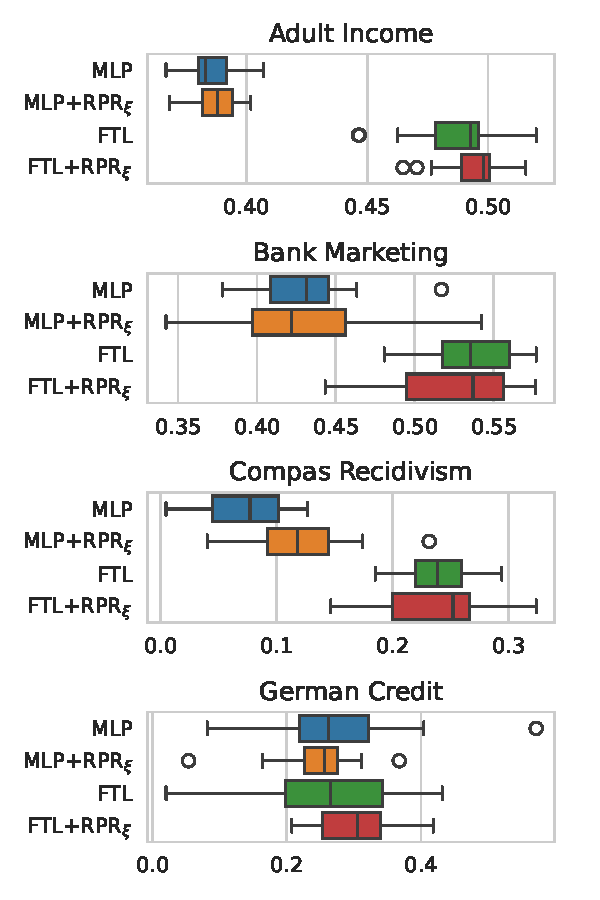
\includegraphics[width=1\linewidth]{images/boxplot_mcc_parity_rpr.pdf}
\end{subfigure}
\begin{subfigure}{.32\linewidth}
    \caption{Equal Opportunity}
    \label{fig:boxplot_mcc_opp_rpr}
    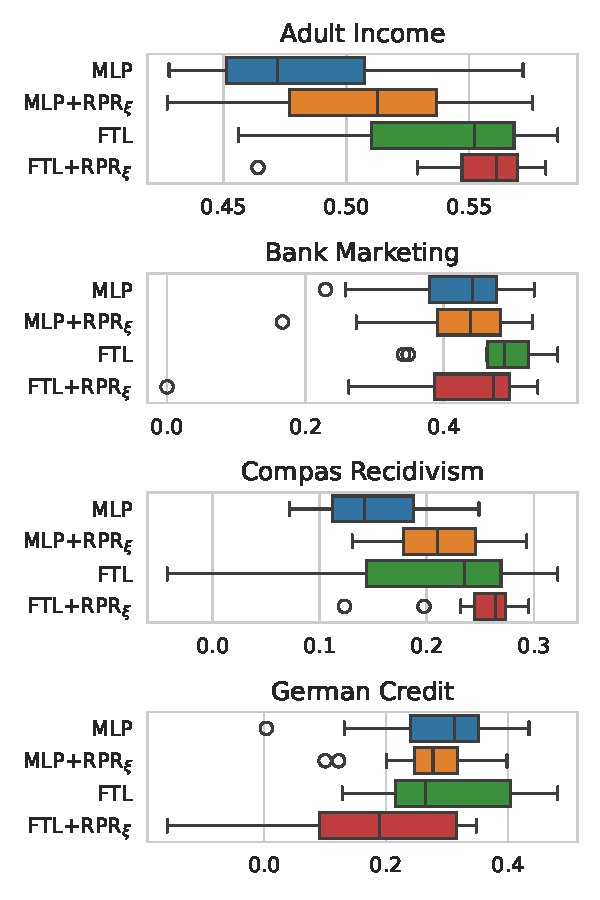
\includegraphics[width=1\linewidth]{images/boxplot_mcc_opportunity_rpr.pdf}
\end{subfigure}
\begin{subfigure}{.32\linewidth}
    \caption{Equalized Odds}
    \label{fig:boxplot_mcc_odds_rpr}
    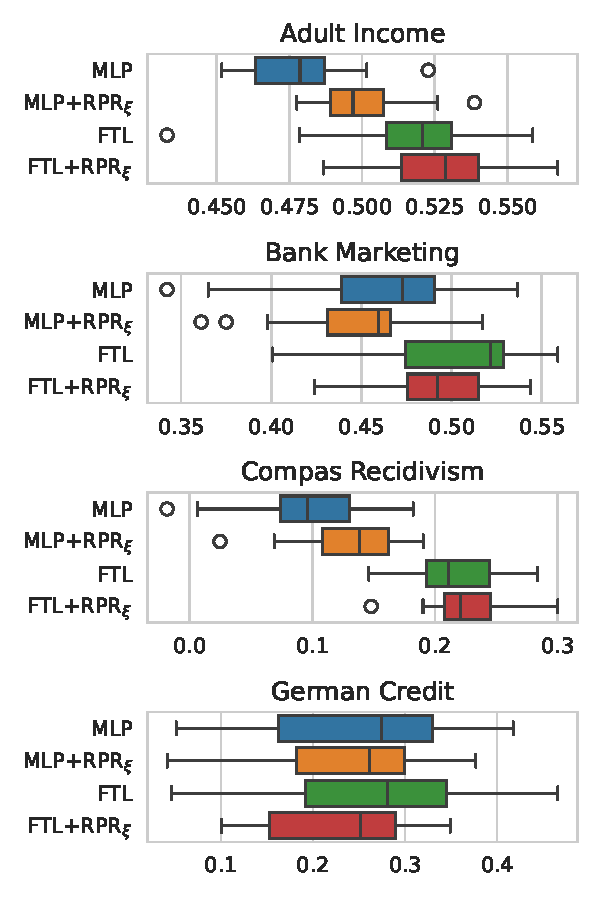
\includegraphics[width=1\linewidth]{images/boxplot_mcc_odds_rpr.pdf}
\end{subfigure}
\end{figure}

\begin{figure}[!ht]
\centering
\caption{Fitness values of RPR optimizing Accuracy and multiple fairness metrics.}\label{fig:boxplot_acc_rpr}
\begin{subfigure}{.32\linewidth}
    \caption{Statistical Parity}
    \label{fig:boxplot_acc_parity_rpr}
    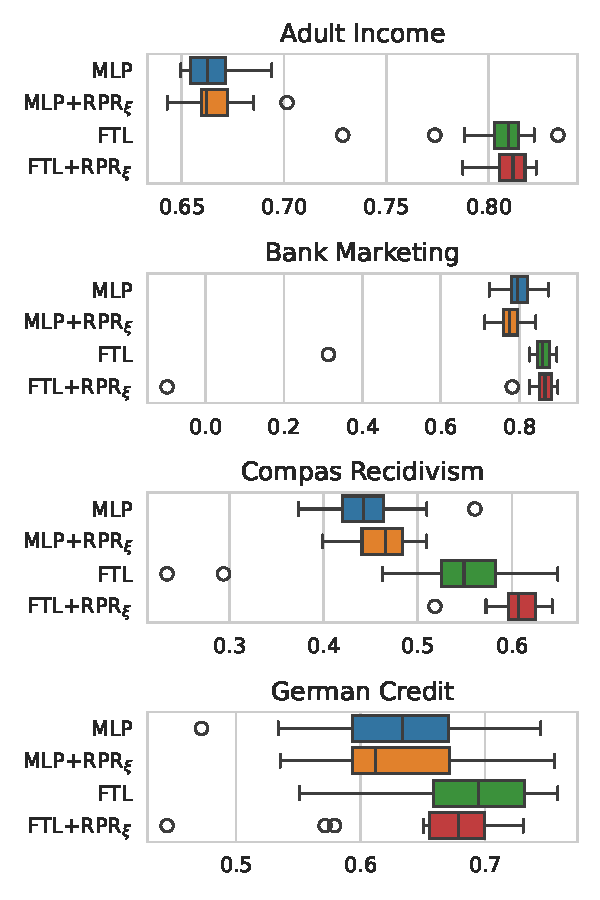
\includegraphics[width=1\linewidth]{images/boxplot_acc_parity_rpr.pdf}
\end{subfigure}
\begin{subfigure}{.32\linewidth}
    \caption{Equal Opportunity}
    \label{fig:boxplot_acc_opp_rpr}
    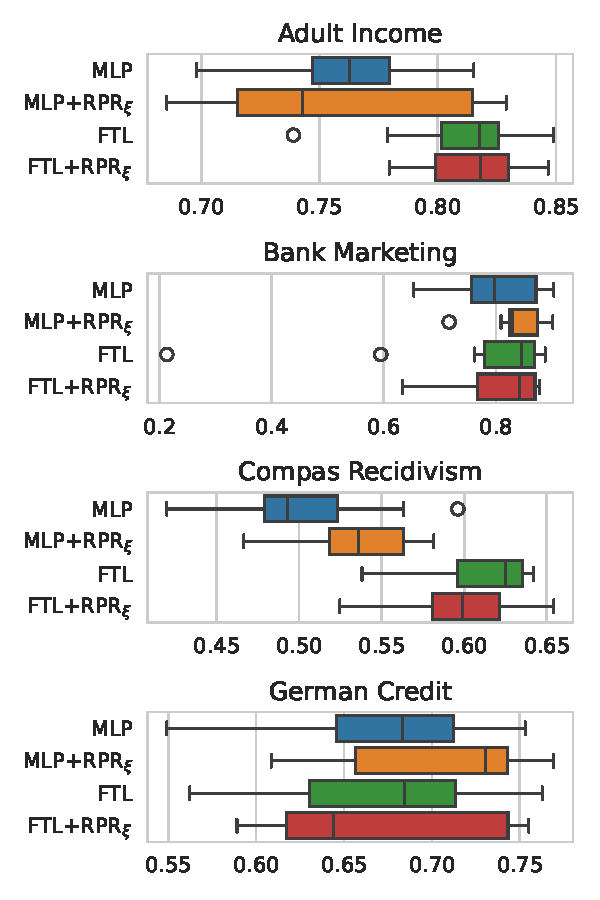
\includegraphics[width=1\linewidth]{images/boxplot_acc_opportunity_rpr.pdf}
\end{subfigure}
\begin{subfigure}{.32\linewidth}
    \caption{Equalized Odds}
    \label{fig:boxplot_acc_odds_rpr}
    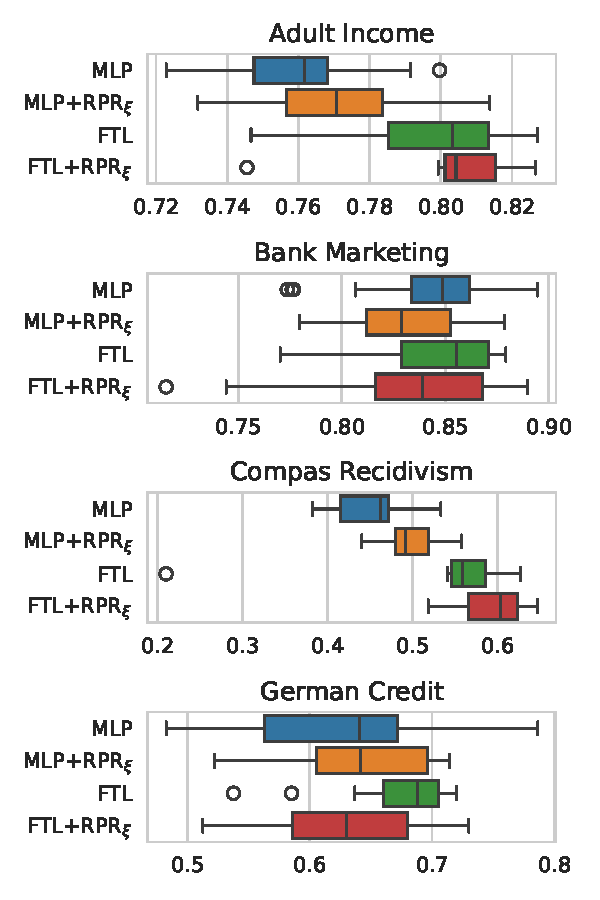
\includegraphics[width=1\linewidth]{images/boxplot_acc_odds_rpr.pdf}
\end{subfigure}
\end{figure}

Now we compare the effects of Redlining Penalty Regularizer on both MLP with standard cross entropy loss and fair transition loss. The MLP baseline here is the same presented on the last comparison (Table~\ref{tab:aso_compare_rpr_variations}), and the FTL model uses the same MLP architecture. The overall methodology remains the same, including $15$ runs with dataset resampling with $100$ trials to hyperparameter tuning each, according Table~\ref{tab:hyperparameters_rpr}. The FTL model without RPR is exactly that same presented at Chapter~\ref{chap:ftl} and on \cite{Canalli2024}, whose achieved state-of-art results. In order to provide a straightforward comparison we include only RPR$_\xi$, as it reaches the best results when compared with the others. The ASO results are available at Table~\ref{tab:aso_compare_rpr} and the box-plot comparison at Figure~\ref{fig:boxplot_mcc_rpr} and Figure~\ref{fig:boxplot_acc_rpr}.

As an additional resource to interpret these results we plot at Figure~\ref{fig:datasets_correlation} the correlations of each feature to the sensitive to each described correlation coefficient at each dataset. The correlation values are presented from highest value to the lower, to provide a non-ascendant visualization. Also, we omit the correlation of sensitive feature to it self (always $1.0$) and plot both the top $10$ correlations and the values to each feature, according the number of features at corresponding dataset. Note that Chatterjee's performs very differently when compared to the others, identifying more highly correlation values, demonstrating the functional relationship of many features with the sensitive and therefore theirs potential to be used as proxy features by the model. Another relevant perception is that the \textit{Bank dataset} presents considerably lower correlations, although still very high values than the others.  

\begin{figure}[!ht]
\centering
\caption{Sorted feature's correlation to the sensitive one according multiple correlation coefficients to all datasets.}\label{fig:datasets_correlation}
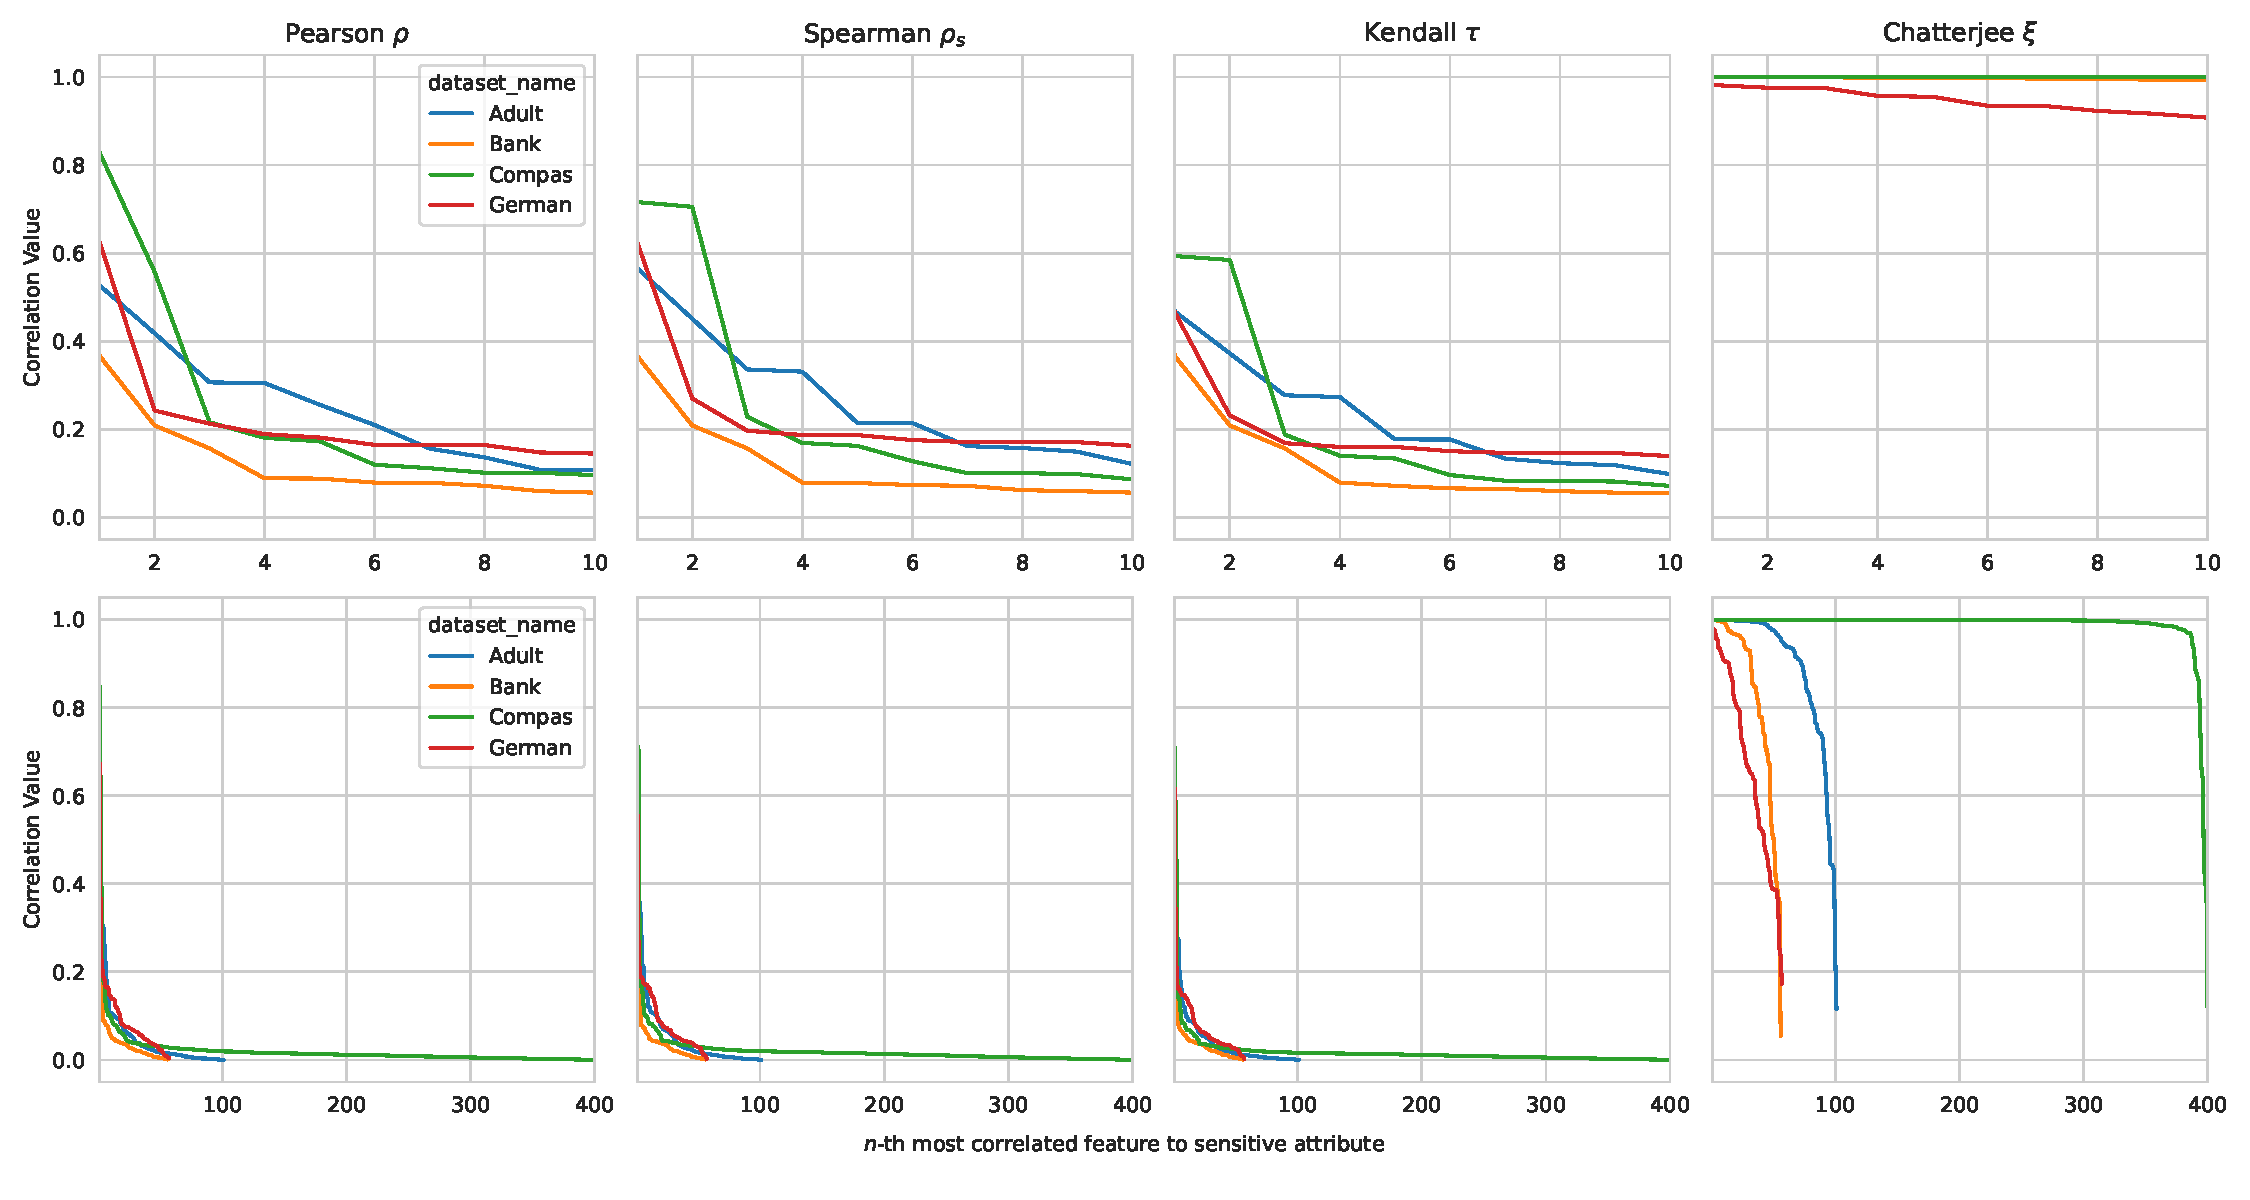
\includegraphics[width=1\linewidth]{images/dataset_correlation_plots.pdf}
\end{figure}

On Table~\ref{tab:aso_compare_rpr} RPR presents low ASO values in many scenarios, on which we can claim that it outperforms the corresponding model without penalty. It is clear that both MLP and FTL benefit with the use of RPR, whose results remains strongly better to most of optimization objectives. Here the main difference is the dataset. While to \textit{Adult} and \textit{COMPAS} the model with RPR consistently outperforms its counterparts, this not happens when the proposed technique is evaluated on \textit{Bank} and \textit{German} datasets. As referred before, \textit{German Credit} is a very small and simple dataset. In this condition the Pareto frontier is rapidly achieved, with no room left for improvement. This condition clear looking at at Figure~\ref{fig:boxplot_mcc_rpr} and Figure~\ref{fig:boxplot_acc_rpr}.  

Additionally, when comparing \textit{Bank}'s features correlations to sensitive at Figure~\ref{fig:datasets_correlation} we can argue that as it presents reduced redlining effect, the effectiveness of the proposed penalty strategy is also reduced. Analogously, the best RPR results are those assessed on \textit{COMPAS}, the dataset with the most aggressive redlining effect.

Thus, on those conditions where the dataset presents features with high potential to be learned as proxy to the sensitive feature by the model, Redlining Penalty Regularizer consistently outperforms the model without regularization. This happens to both MLP models, the one using standard cross entropy loss and with Fair Transition Loss. In this last scenario the state-of-art results described before are enhanced.

As done on the last chapter, we present performance and fairness results along with the fitness, in order to provide material to a trade-off analysis. Those metric values enable the reader to compare this results with different experimental setup and fitness objective from literature. Results corresponding each optimization scenario can be found on tables \ref{tab:complete_mcc_parity_rpr} to \ref{tab:complete_acc_odds_rpr}, presenting metric means and standard deviation values across multiple resample run. Best result of each metric within evaluation scenario are in bold, and standard deviation values are presented between parenthesis. Up arrow ($\uparrow$) indicates that the referred metric should be maximized while down arrow ($\downarrow$) that the metric should be minimized. To provide a visual resource to this comparison, the distribution of those metrics across multiple resample runs comparing the Redlining Penalty Regularization using Chatterjee's correlation (FTL) on baseline (MLP) and Fair Transition Loss (FTL) are presented in joint plot format in figures \ref{fig:complete_mcc_parity_rpr} to \ref{fig:complete_acc_odds_rpr}. Each joint plot is present within the corresponding table to a better comprehension.

\newpage

\begin{table}
    \centering
    \caption{Mean and standard deviation metric values optimizing MCC and Statistical Parity in comparison with Redlining Penalty Regularizer.}\label{tab:complete_mcc_parity_rpr}
    {\tiny\begin{tabular}{llrrr}
    \toprule
    Dataset & Method & $\uparrow\;$Fitness & $\uparrow\;$MCC & $\downarrow\;$Stat. Parity \\
    \midrule
    \multirow{8}{*}{\shortstack[l]{Adult\\ Income}} & FTL & $0.487 \; (\pm0.02)$ & $0.509 \; (\pm0.02)$ & $\textbf{0.022} \; (\pm0.02)$ \\
     & FTL+RPR$_{\xi}$ & $\textbf{0.494} \; (\pm0.01)$ & $0.517 \; (\pm0.02)$ & $0.023 \; (\pm0.02)$ \\
     & MLP & $0.386 \; (\pm0.01)$ & $0.576 \; (\pm0.01)$ & $0.191 \; (\pm0.01)$ \\
     & MLP+L2 & $0.385 \; (\pm0.01)$ & $0.576 \; (\pm0.01)$ & $0.190 \; (\pm0.01)$ \\
     & MLP+RPR$_{\rho_s}$ & $0.384 \; (\pm0.01)$ & $0.576 \; (\pm0.01)$ & $0.192 \; (\pm0.01)$ \\
     & MLP+RPR$_{\rho}$ & $0.393 \; (\pm0.01)$ & $\textbf{0.580} \; (\pm0.01)$ & $0.187 \; (\pm0.01)$ \\
     & MLP+RPR$_{\tau}$ & $0.386 \; (\pm0.01)$ & $0.577 \; (\pm0.01)$ & $0.191 \; (\pm0.01)$ \\
     & MLP+RPR$_{\xi}$ & $0.388 \; (\pm0.01)$ & $0.578 \; (\pm0.01)$ & $0.191 \; (\pm0.01)$ \\
    \midrule
    \multirow{8}{*}{\shortstack[l]{Bank\\ Marketing}} & FTL & $\textbf{0.534} \; (\pm0.03)$ & $\textbf{0.569} \; (\pm0.01)$ & $\textbf{0.035} \; (\pm0.03)$ \\
     & FTL+RPR$_{\xi}$ & $0.523 \; (\pm0.04)$ & $\textbf{0.569} \; (\pm0.01)$ & $0.046 \; (\pm0.04)$ \\
     & MLP & $0.429 \; (\pm0.03)$ & $0.521 \; (\pm0.02)$ & $0.092 \; (\pm0.02)$ \\
     & MLP+L2 & $0.412 \; (\pm0.04)$ & $0.521 \; (\pm0.02)$ & $0.110 \; (\pm0.03)$ \\
     & MLP+RPR$_{\rho_s}$ & $0.422 \; (\pm0.03)$ & $0.527 \; (\pm0.02)$ & $0.106 \; (\pm0.03)$ \\
     & MLP+RPR$_{\rho}$ & $0.424 \; (\pm0.03)$ & $0.523 \; (\pm0.01)$ & $0.100 \; (\pm0.03)$ \\
     & MLP+RPR$_{\tau}$ & $0.412 \; (\pm0.04)$ & $0.520 \; (\pm0.02)$ & $0.108 \; (\pm0.03)$ \\
     & MLP+RPR$_{\xi}$ & $0.426 \; (\pm0.05)$ & $0.528 \; (\pm0.02)$ & $0.102 \; (\pm0.04)$ \\
    \midrule
    \multirow{8}{*}{\shortstack[l]{COMPAS\\ Recidivism}} & FTL & $\textbf{0.239} \; (\pm0.03)$ & $0.276 \; (\pm0.03)$ & $\textbf{0.036} \; (\pm0.03)$ \\
     & FTL+RPR$_{\xi}$ & $0.236 \; (\pm0.05)$ & $0.294 \; (\pm0.03)$ & $0.058 \; (\pm0.04)$ \\
     & MLP & $0.074 \; (\pm0.03)$ & $0.283 \; (\pm0.02)$ & $0.209 \; (\pm0.04)$ \\
     & MLP+L2 & $0.089 \; (\pm0.04)$ & $0.291 \; (\pm0.02)$ & $0.202 \; (\pm0.04)$ \\
     & MLP+RPR$_{\rho_s}$ & $0.083 \; (\pm0.05)$ & $0.293 \; (\pm0.03)$ & $0.210 \; (\pm0.04)$ \\
     & MLP+RPR$_{\rho}$ & $0.087 \; (\pm0.05)$ & $0.282 \; (\pm0.03)$ & $0.195 \; (\pm0.04)$ \\
     & MLP+RPR$_{\tau}$ & $0.085 \; (\pm0.03)$ & $0.281 \; (\pm0.02)$ & $0.197 \; (\pm0.03)$ \\
     & MLP+RPR$_{\xi}$ & $0.121 \; (\pm0.05)$ & $\textbf{0.329} \; (\pm0.03)$ & $0.208 \; (\pm0.03)$ \\
    \midrule
    \multirow{8}{*}{\shortstack[l]{German\\ Credit}} & FTL & $0.256 \; (\pm0.12)$ & $0.355 \; (\pm0.08)$ & $0.099 \; (\pm0.06)$ \\
     & FTL+RPR$_{\xi}$ & $\textbf{0.302} \; (\pm0.06)$ & $0.371 \; (\pm0.05)$ & $0.069 \; (\pm0.05)$ \\
     & MLP & $0.266 \; (\pm0.10)$ & $0.329 \; (\pm0.09)$ & $\textbf{0.064} \; (\pm0.05)$ \\
     & MLP+L2 & $0.261 \; (\pm0.10)$ & $\textbf{0.374} \; (\pm0.09)$ & $0.113 \; (\pm0.07)$ \\
     & MLP+RPR$_{\rho_s}$ & $0.192 \; (\pm0.11)$ & $0.292 \; (\pm0.07)$ & $0.099 \; (\pm0.06)$ \\
     & MLP+RPR$_{\rho}$ & $0.255 \; (\pm0.07)$ & $0.341 \; (\pm0.07)$ & $0.087 \; (\pm0.04)$ \\
     & MLP+RPR$_{\tau}$ & $0.256 \; (\pm0.08)$ & $0.342 \; (\pm0.05)$ & $0.086 \; (\pm0.06)$ \\
     & MLP+RPR$_{\xi}$ & $0.246 \; (\pm0.07)$ & $0.329 \; (\pm0.05)$ & $0.084 \; (\pm0.06)$ \\
    \bottomrule
\end{tabular}}
\end{table}

\begin{figure}
\centering
\caption{Metric distribution optimizing MCC and Statistical Parity in comparison with Redlining Penalty Regularization across multiple resample runs. Corresponding values available at Table~\ref{tab:complete_mcc_parity_rpr}.}
\label{fig:complete_mcc_parity_rpr}
\begin{subfigure}{.45\linewidth}
    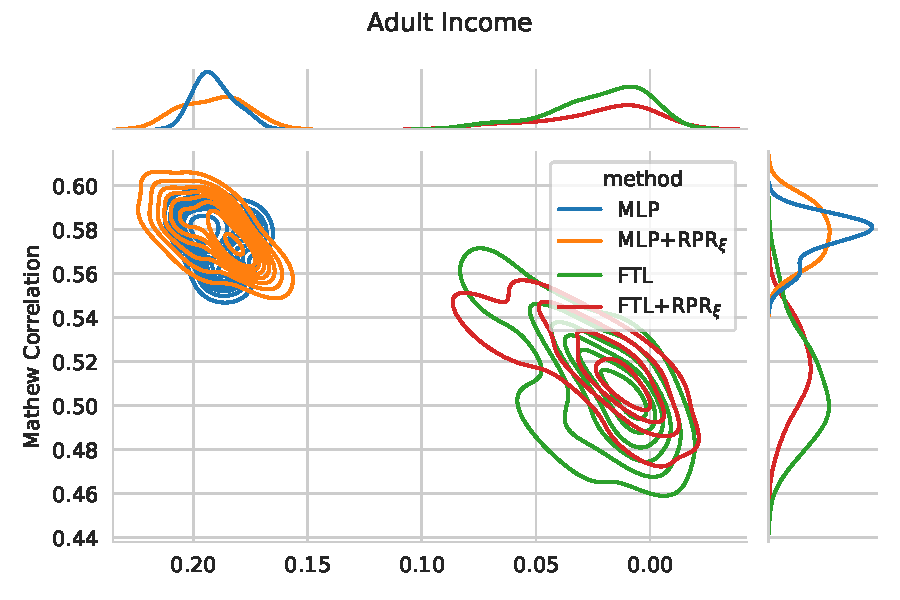
\includegraphics[width=1\linewidth]{images/pareto_mcc_parity_adult_rpr.pdf}
\end{subfigure}
\begin{subfigure}{.45\linewidth}
    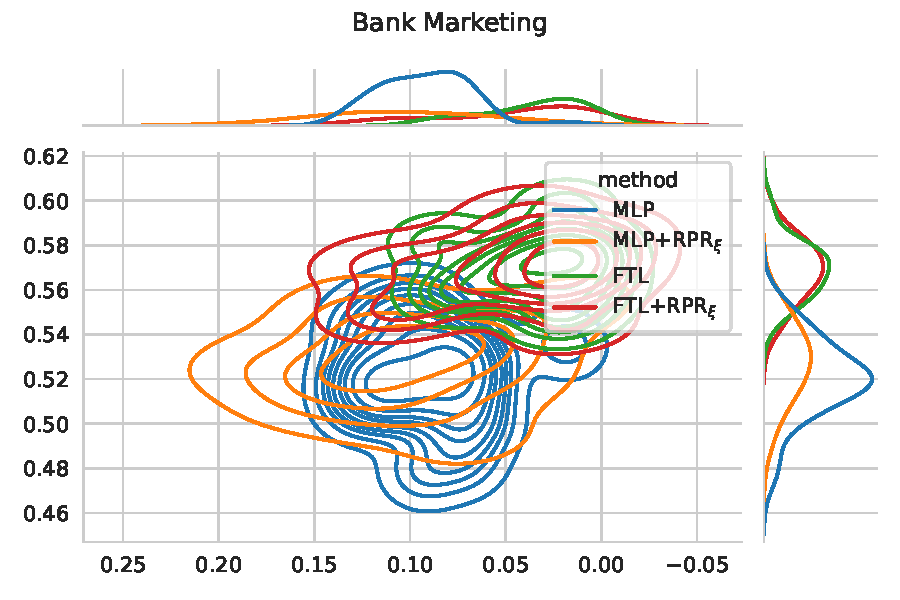
\includegraphics[width=1\linewidth]{images/pareto_mcc_parity_bank_rpr.pdf}
\end{subfigure}

\begin{subfigure}{.45\linewidth}
    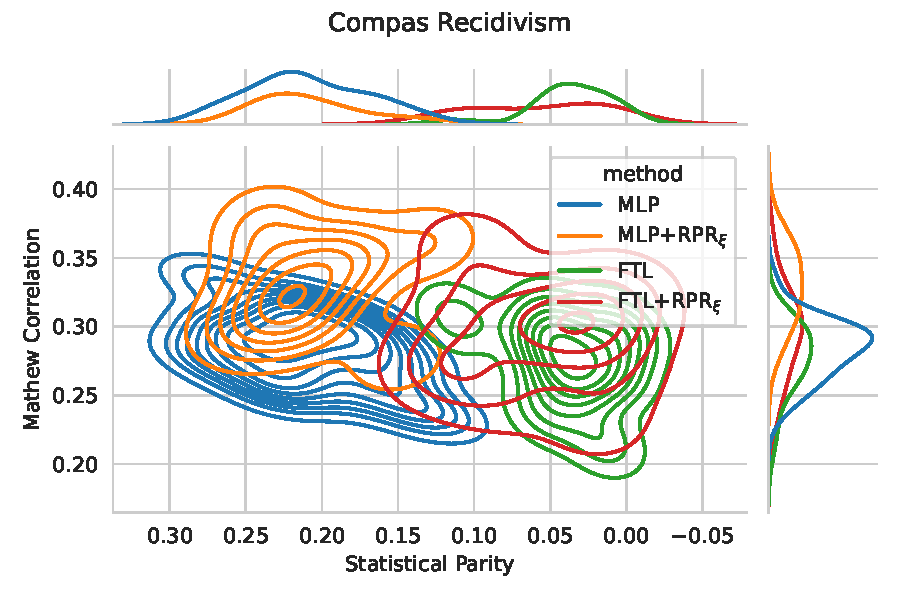
\includegraphics[width=1\linewidth]{images/pareto_mcc_parity_compas_rpr.pdf}
\end{subfigure}
\begin{subfigure}{.45\linewidth}
    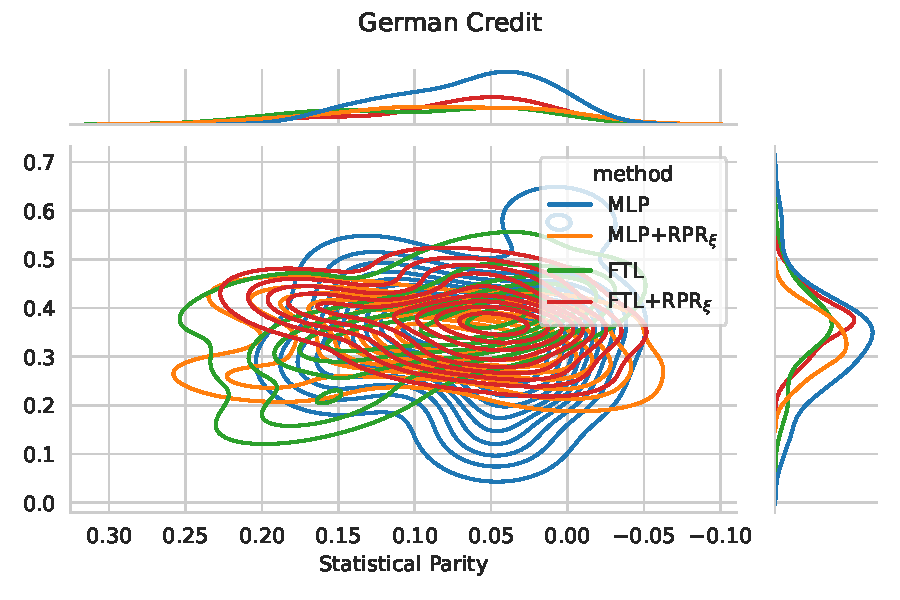
\includegraphics[width=1\linewidth]{images/pareto_mcc_parity_german_rpr.pdf}
\end{subfigure}
\end{figure}

 \begin{table}
    \centering
    \caption{Mean and standard deviation metric values optimizing MCC and Equal Opportunity in comparison with Redlining Penalty Regularizer.}\label{tab:complete_mcc_opportunity_rpr}
    {\tiny\begin{tabular}{llrrr}
    \toprule
    Dataset & Method & $\uparrow\;$Fitness & $\uparrow\;$MCC & $\downarrow\;$Eq. Opp. \\
    \midrule
    
    \multirow{8}{*}{\shortstack[l]{Adult\\ Income}} & FTL & $0.540 \; (\pm0.04)$ & $0.576 \; (\pm0.01)$ & $0.036 \; (\pm0.03)$ \\
     & FTL+RPR$_{\xi}$ & $\textbf{0.554} \; (\pm0.03)$ & $0.581 \; (\pm0.02)$ & $\textbf{0.027} \; (\pm0.02)$ \\
     & MLP & $0.480 \; (\pm0.04)$ & $\textbf{0.582} \; (\pm0.01)$ & $0.103 \; (\pm0.04)$ \\
     & MLP+L2 & $0.479 \; (\pm0.03)$ & $0.580 \; (\pm0.01)$ & $0.102 \; (\pm0.03)$ \\
     & MLP+RPR$_{\rho_s}$ & $0.493 \; (\pm0.04)$ & $0.578 \; (\pm0.01)$ & $0.085 \; (\pm0.04)$ \\
     & MLP+RPR$_{\rho}$ & $0.478 \; (\pm0.04)$ & $0.580 \; (\pm0.01)$ & $0.102 \; (\pm0.04)$ \\
     & MLP+RPR$_{\tau}$ & $0.488 \; (\pm0.04)$ & $0.580 \; (\pm0.01)$ & $0.092 \; (\pm0.03)$ \\
     & MLP+RPR$_{\xi}$ & $0.506 \; (\pm0.05)$ & $0.577 \; (\pm0.01)$ & $0.071 \; (\pm0.05)$ \\
    \midrule
    \multirow{8}{*}{\shortstack[l]{Bank\\ Marketing}} & FTL & $\textbf{0.483} \; (\pm0.07)$ & $\textbf{0.567} \; (\pm0.02)$ & $0.084 \; (\pm0.06)$ \\
     & FTL+RPR$_{\xi}$ & $0.416 \; (\pm0.14)$ & $0.519 \; (\pm0.15)$ & $0.104 \; (\pm0.08)$ \\
     & MLP & $0.420 \; (\pm0.08)$ & $0.524 \; (\pm0.02)$ & $0.104 \; (\pm0.08)$ \\
     & MLP+L2 & $0.438 \; (\pm0.06)$ & $0.514 \; (\pm0.02)$ & $0.076 \; (\pm0.06)$ \\
     & MLP+RPR$_{\rho_s}$ & $0.426 \; (\pm0.06)$ & $0.520 \; (\pm0.02)$ & $0.094 \; (\pm0.06)$ \\
     & MLP+RPR$_{\rho}$ & $0.452 \; (\pm0.05)$ & $0.527 \; (\pm0.02)$ & $\textbf{0.074} \; (\pm0.05)$ \\
     & MLP+RPR$_{\tau}$ & $0.417 \; (\pm0.08)$ & $0.526 \; (\pm0.02)$ & $0.109 \; (\pm0.07)$ \\
     & MLP+RPR$_{\xi}$ & $0.420 \; (\pm0.10)$ & $0.529 \; (\pm0.02)$ & $0.109 \; (\pm0.09)$ \\
    \midrule
    \multirow{8}{*}{\shortstack[l]{COMPAS\\ Recidivism}} & FTL & $0.195 \; (\pm0.11)$ & $0.281 \; (\pm0.03)$ & $0.086 \; (\pm0.09)$ \\
     & FTL+RPR$_{\xi}$ & $\textbf{0.251} \; (\pm0.04)$ & $0.309 \; (\pm0.03)$ & $\textbf{0.058} \; (\pm0.04)$ \\
     & MLP & $0.150 \; (\pm0.05)$ & $0.282 \; (\pm0.03)$ & $0.132 \; (\pm0.05)$ \\
     & MLP+L2 & $0.146 \; (\pm0.06)$ & $0.282 \; (\pm0.03)$ & $0.136 \; (\pm0.04)$ \\
     & MLP+RPR$_{\rho_s}$ & $0.179 \; (\pm0.04)$ & $0.303 \; (\pm0.02)$ & $0.124 \; (\pm0.03)$ \\
     & MLP+RPR$_{\rho}$ & $0.168 \; (\pm0.06)$ & $0.290 \; (\pm0.03)$ & $0.122 \; (\pm0.05)$ \\
     & MLP+RPR$_{\tau}$ & $0.146 \; (\pm0.05)$ & $0.289 \; (\pm0.03)$ & $0.143 \; (\pm0.04)$ \\
     & MLP+RPR$_{\xi}$ & $0.211 \; (\pm0.05)$ & $\textbf{0.325} \; (\pm0.02)$ & $0.114 \; (\pm0.04)$ \\
    \midrule
    \multirow{8}{*}{\shortstack[l]{German\\ Credit}} & FTL & $\textbf{0.293} \; (\pm0.12)$ & $\textbf{0.368} \; (\pm0.10)$ & $0.074 \; (\pm0.05)$ \\
     & FTL+RPR$_{\xi}$ & $0.166 \; (\pm0.16)$ & $0.284 \; (\pm0.14)$ & $0.117 \; (\pm0.07)$ \\
     & MLP & $0.290 \; (\pm0.09)$ & $0.355 \; (\pm0.07)$ & $0.065 \; (\pm0.06)$ \\
     & MLP+L2 & $0.249 \; (\pm0.08)$ & $0.309 \; (\pm0.07)$ & $0.060 \; (\pm0.04)$ \\
     & MLP+RPR$_{\rho_s}$ & $0.319 \; (\pm0.05)$ & $0.367 \; (\pm0.07)$ & $\textbf{0.048} \; (\pm0.04)$ \\
     & MLP+RPR$_{\rho}$ & $0.229 \; (\pm0.13)$ & $0.297 \; (\pm0.10)$ & $0.068 \; (\pm0.04)$ \\
     & MLP+RPR$_{\tau}$ & $0.277 \; (\pm0.08)$ & $0.329 \; (\pm0.06)$ & $0.053 \; (\pm0.04)$ \\
     & MLP+RPR$_{\xi}$ & $0.275 \; (\pm0.09)$ & $0.341 \; (\pm0.06)$ & $0.066 \; (\pm0.05)$ \\
     \bottomrule
\end{tabular}}
\end{table}

\begin{figure}
\centering
\caption{Metric distribution optimizing MCC and Equal Opportunity in comparison with Redlining Penalty Regularization across multiple resample runs. Corresponding values available at Table~\ref{tab:complete_mcc_opportunity_rpr}.}
\label{fig:complete_mcc_opportunity_rpr}
\begin{subfigure}{.45\linewidth}
    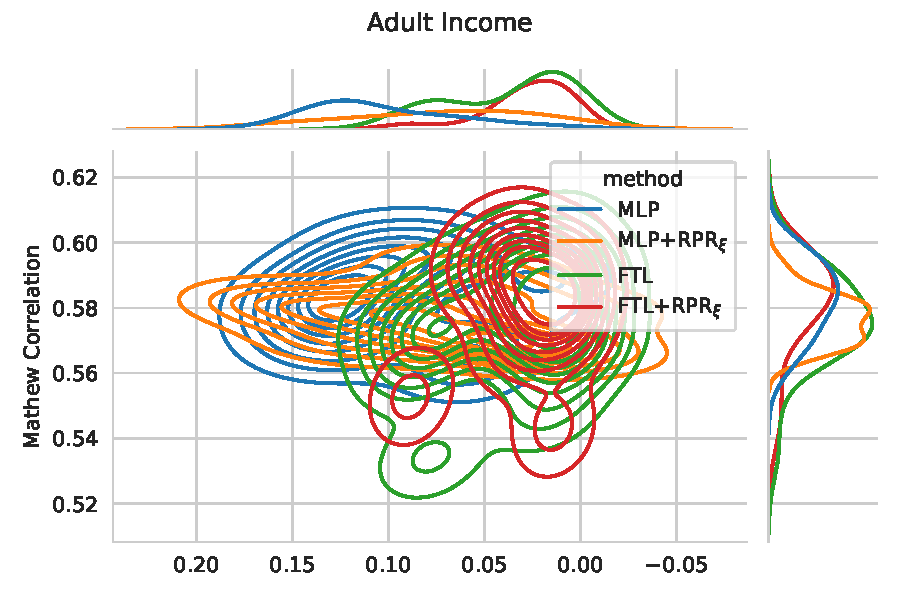
\includegraphics[width=1\linewidth]{images/pareto_mcc_opportunity_adult_rpr.pdf}
\end{subfigure}
\begin{subfigure}{.45\linewidth}
    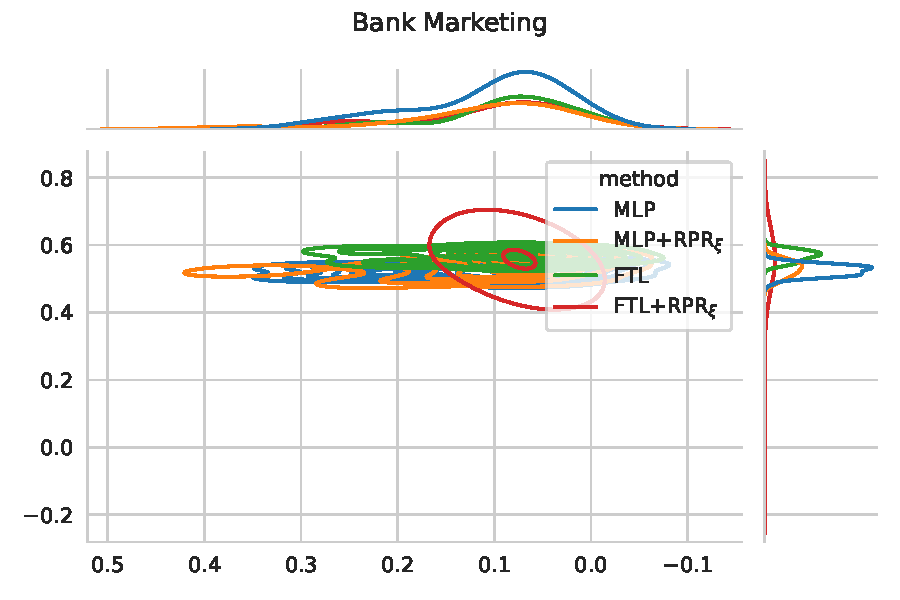
\includegraphics[width=1\linewidth]{images/pareto_mcc_opportunity_bank_rpr.pdf}
\end{subfigure}

\begin{subfigure}{.45\linewidth}
    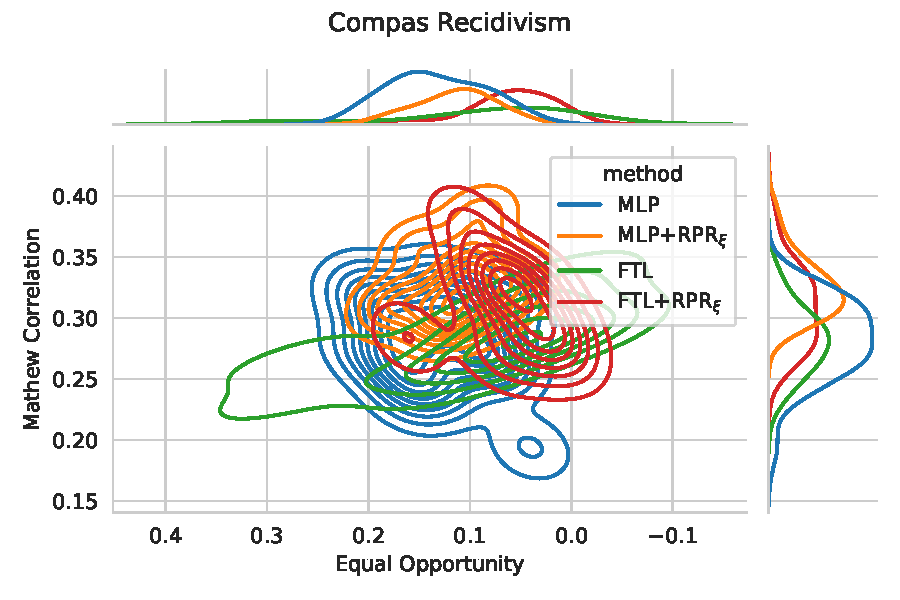
\includegraphics[width=1\linewidth]{images/pareto_mcc_opportunity_compas_rpr.pdf}
\end{subfigure}
\begin{subfigure}{.45\linewidth}
    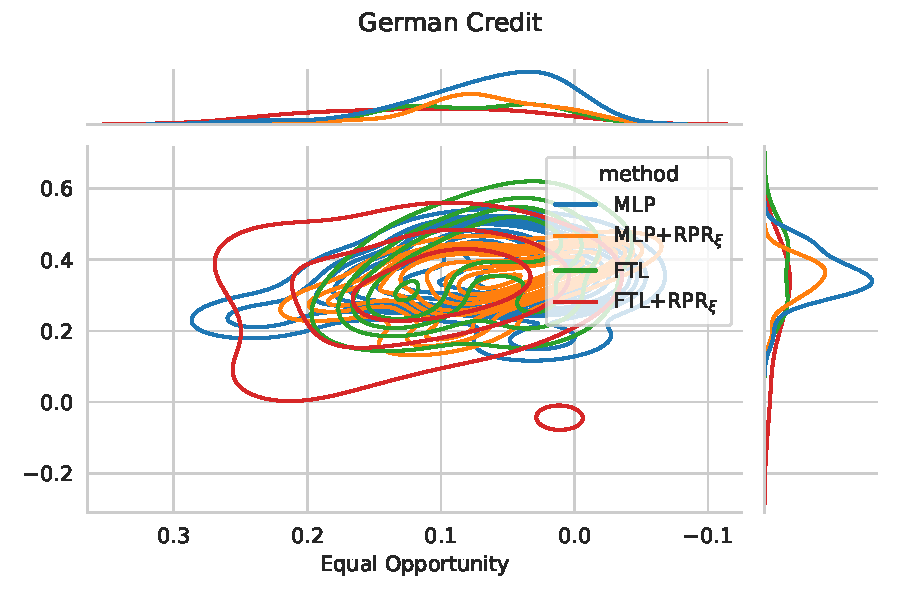
\includegraphics[width=1\linewidth]{images/pareto_mcc_opportunity_german_rpr.pdf}
\end{subfigure}
\end{figure}


 \begin{table}
    \centering
    \caption{Mean and standard deviation metric values optimizing MCC and Equalized Odds in comparison with Redlining Penalty Regularizer.}\label{tab:complete_mcc_odds_rpr}
    {\tiny\begin{tabular}{llrrr}
    \toprule
    Dataset & Method & $\uparrow\;$Fitness & $\uparrow\;$MCC & $\downarrow\;$Eq. Odds \\
    \midrule
    
    \multirow{8}{*}{\shortstack[l]{Adult\\ Income}} & FTL & $0.515 \; (\pm0.03)$ & $0.572 \; (\pm0.02)$ & $0.057 \; (\pm0.02)$ \\
     & FTL+RPR$_{\xi}$ & $\textbf{0.526} \; (\pm0.02)$ & $0.575 \; (\pm0.01)$ & $\textbf{0.048} \; (\pm0.02)$ \\
     & MLP & $0.478 \; (\pm0.02)$ & $0.575 \; (\pm0.01)$ & $0.097 \; (\pm0.02)$ \\
     & MLP+L2 & $0.484 \; (\pm0.01)$ & $0.577 \; (\pm0.01)$ & $0.093 \; (\pm0.01)$ \\
     & MLP+RPR$_{\rho_s}$ & $0.492 \; (\pm0.02)$ & $\textbf{0.578} \; (\pm0.01)$ & $0.085 \; (\pm0.02)$ \\
     & MLP+RPR$_{\rho}$ & $0.489 \; (\pm0.02)$ & $0.575 \; (\pm0.01)$ & $0.087 \; (\pm0.02)$ \\
     & MLP+RPR$_{\tau}$ & $0.487 \; (\pm0.02)$ & $\textbf{0.578} \; (\pm0.01)$ & $0.091 \; (\pm0.02)$ \\
     & MLP+RPR$_{\xi}$ & $0.500 \; (\pm0.02)$ & $\textbf{0.578} \; (\pm0.01)$ & $0.078 \; (\pm0.02)$ \\
    \midrule
    \multirow{8}{*}{\shortstack[l]{Bank\\ Marketing}} & FTL & $\textbf{0.495} \; (\pm0.05)$ & $\textbf{0.574} \; (\pm0.01)$ & $0.078 \; (\pm0.05)$ \\
     & FTL+RPR$_{\xi}$ & $0.490 \; (\pm0.03)$ & $0.571 \; (\pm0.01)$ & $0.081 \; (\pm0.03)$ \\
     & MLP & $0.461 \; (\pm0.05)$ & $0.522 \; (\pm0.02)$ & $\textbf{0.061} \; (\pm0.04)$ \\
     & MLP+L2 & $0.461 \; (\pm0.03)$ & $0.525 \; (\pm0.02)$ & $0.065 \; (\pm0.03)$ \\
     & MLP+RPR$_{\rho_s}$ & $0.468 \; (\pm0.04)$ & $0.529 \; (\pm0.02)$ & $\textbf{0.061} \; (\pm0.03)$ \\
     & MLP+RPR$_{\rho}$ & $0.442 \; (\pm0.05)$ & $0.522 \; (\pm0.02)$ & $0.080 \; (\pm0.03)$ \\
     & MLP+RPR$_{\tau}$ & $0.434 \; (\pm0.05)$ & $0.519 \; (\pm0.01)$ & $0.085 \; (\pm0.05)$ \\
     & MLP+RPR$_{\xi}$ & $0.446 \; (\pm0.04)$ & $0.539 \; (\pm0.02)$ & $0.093 \; (\pm0.04)$ \\
    \midrule
    \multirow{8}{*}{\shortstack[l]{COMPAS\\ Recidivism}} & FTL & $0.216 \; (\pm0.04)$ & $0.288 \; (\pm0.02)$ & $0.072 \; (\pm0.04)$ \\
     & FTL+RPR$_{\xi}$ & $\textbf{0.225} \; (\pm0.04)$ & $0.282 \; (\pm0.03)$ & $\textbf{0.056} \; (\pm0.03)$ \\
     & MLP & $0.098 \; (\pm0.05)$ & $0.283 \; (\pm0.03)$ & $0.185 \; (\pm0.03)$ \\
     & MLP+L2 & $0.097 \; (\pm0.04)$ & $0.281 \; (\pm0.03)$ & $0.185 \; (\pm0.04)$ \\
     & MLP+RPR$_{\rho_s}$ & $0.096 \; (\pm0.05)$ & $0.282 \; (\pm0.03)$ & $0.185 \; (\pm0.03)$ \\
     & MLP+RPR$_{\rho}$ & $0.119 \; (\pm0.05)$ & $0.292 \; (\pm0.03)$ & $0.174 \; (\pm0.03)$ \\
     & MLP+RPR$_{\tau}$ & $0.124 \; (\pm0.04)$ & $\textbf{0.310} \; (\pm0.02)$ & $0.185 \; (\pm0.03)$ \\
     & MLP+RPR$_{\xi}$ & $0.129 \; (\pm0.05)$ & $0.303 \; (\pm0.02)$ & $0.174 \; (\pm0.03)$ \\
    \midrule
    \multirow{8}{*}{\shortstack[l]{German\\ Credit}} & FTL & $\textbf{0.278} \; (\pm0.12)$ & $\textbf{0.383} \; (\pm0.08)$ & $0.105 \; (\pm0.06)$ \\
     & FTL+RPR$_{\xi}$ & $0.228 \; (\pm0.08)$ & $0.337 \; (\pm0.07)$ & $0.109 \; (\pm0.06)$ \\
     & MLP & $0.249 \; (\pm0.10)$ & $0.352 \; (\pm0.08)$ & $0.102 \; (\pm0.06)$ \\
     & MLP+L2 & $0.214 \; (\pm0.11)$ & $0.297 \; (\pm0.10)$ & $\textbf{0.084} \; (\pm0.05)$ \\
     & MLP+RPR$_{\rho_s}$ & $0.219 \; (\pm0.09)$ & $0.352 \; (\pm0.07)$ & $0.133 \; (\pm0.05)$ \\
     & MLP+RPR$_{\rho}$ & $0.228 \; (\pm0.11)$ & $0.342 \; (\pm0.06)$ & $0.114 \; (\pm0.09)$ \\
     & MLP+RPR$_{\tau}$ & $0.247 \; (\pm0.06)$ & $0.341 \; (\pm0.06)$ & $0.094 \; (\pm0.05)$ \\
     & MLP+RPR$_{\xi}$ & $0.231 \; (\pm0.10)$ & $0.332 \; (\pm0.07)$ & $0.102 \; (\pm0.06)$ \\
     \bottomrule
\end{tabular}}
\end{table}

\begin{figure}
\centering
\caption{Metric distribution optimizing MCC and Equalized Odds in comparison with Redlining Penalty Regularization across multiple resample runs. Corresponding values available at Table~\ref{tab:complete_mcc_odds_rpr}.}
\label{fig:complete_mcc_odds_rpr}
\begin{subfigure}{.45\linewidth}
    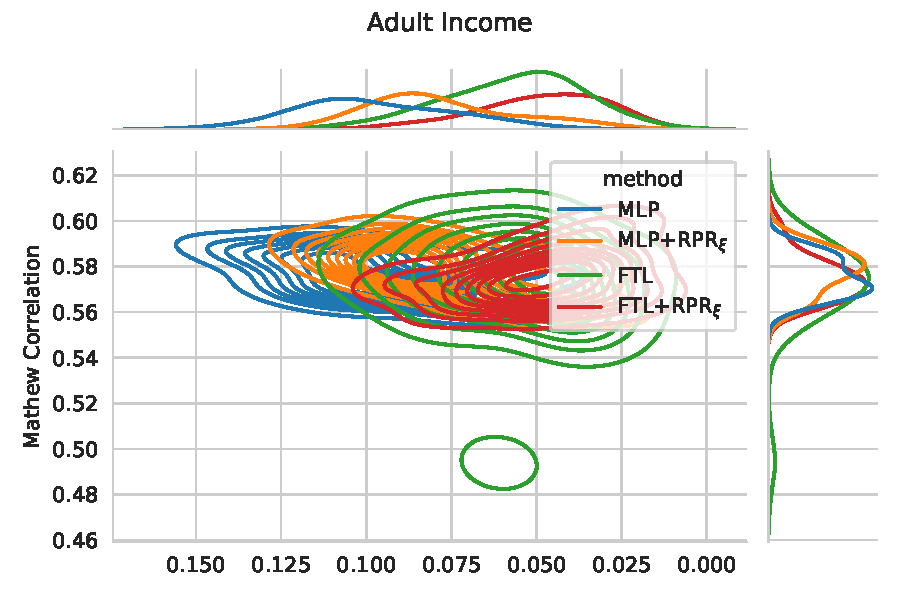
\includegraphics[width=1\linewidth]{images/pareto_mcc_odds_adult_rpr.pdf}
\end{subfigure}
\begin{subfigure}{.45\linewidth}
    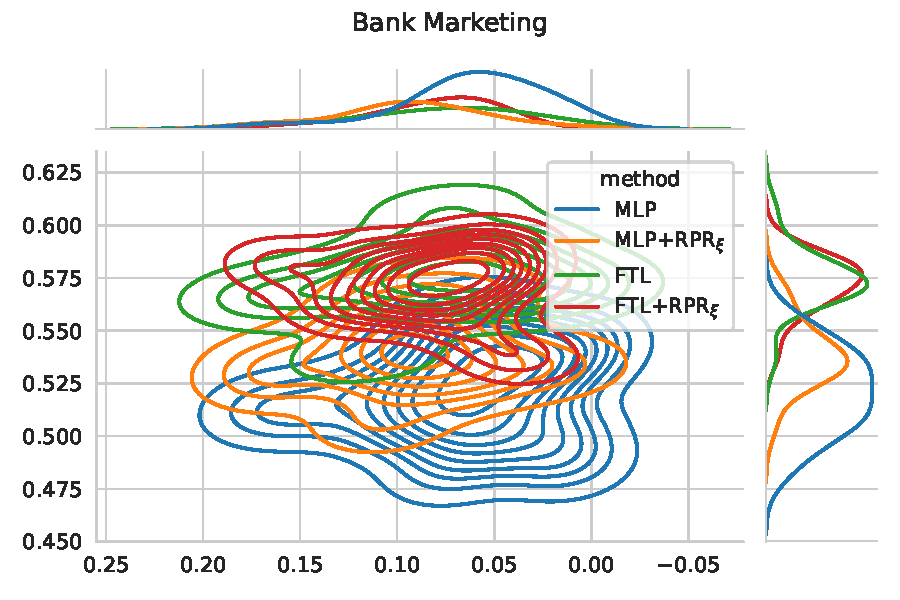
\includegraphics[width=1\linewidth]{images/pareto_mcc_odds_bank_rpr.pdf}
\end{subfigure}

\begin{subfigure}{.45\linewidth}
    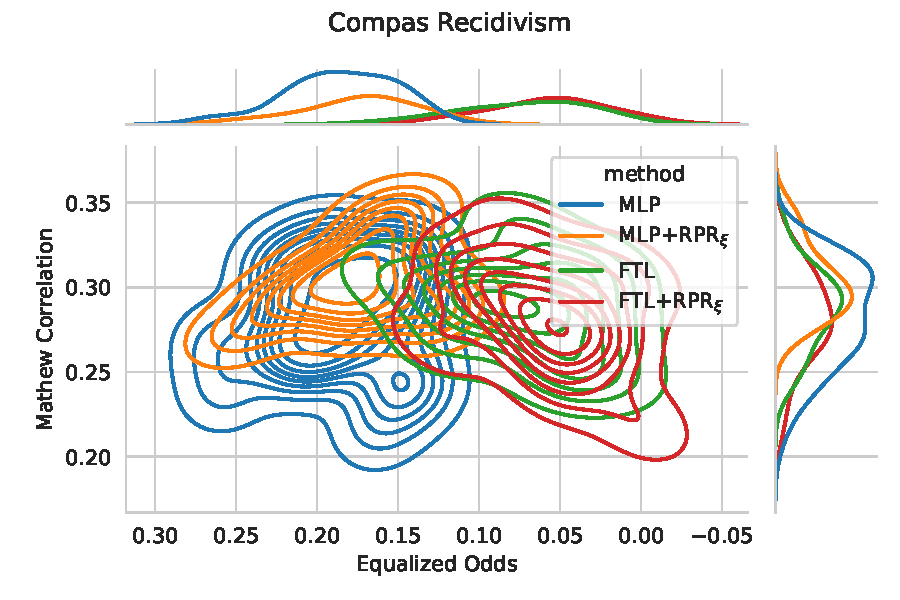
\includegraphics[width=1\linewidth]{images/pareto_mcc_odds_compas_rpr.pdf}
\end{subfigure}
\begin{subfigure}{.45\linewidth}
    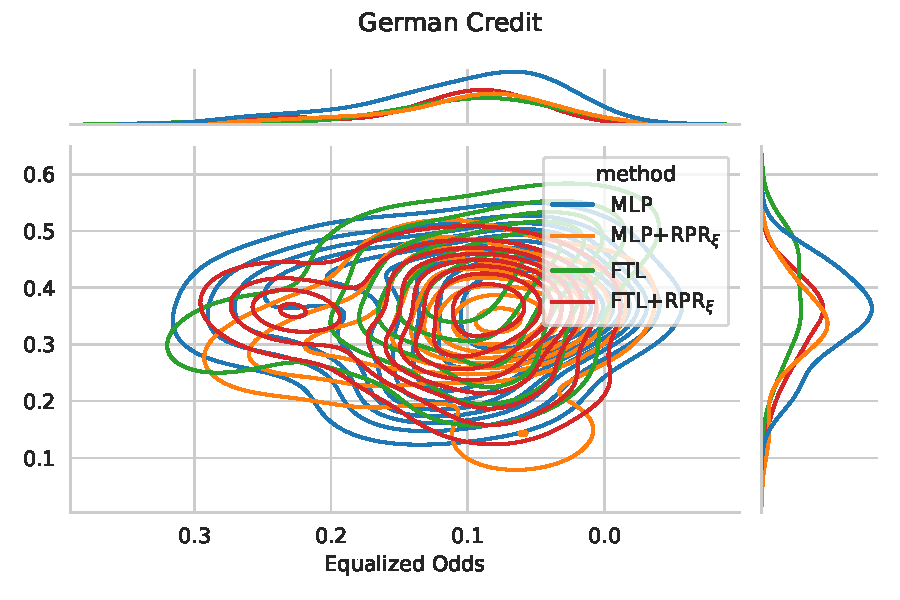
\includegraphics[width=1\linewidth]{images/pareto_mcc_odds_german_rpr.pdf}
\end{subfigure}
\end{figure}

 \begin{table}
    \centering
    \caption{Mean and standard deviation metric values optimizing Accuracy and Statistical Parity in comparison with Redlining Penalty Regularizer.}\label{tab:complete_acc_parity_rpr}
   {\tiny \begin{tabular}{llrrr}
    \toprule
    Dataset & Method & $\uparrow\;$Fitness & $\uparrow\;$Accuracy & $\downarrow\;$Stat. Parity \\
    \midrule
    
    \multirow{8}{*}{\shortstack[l]{Adult\\ Income}} & FTL & $0.806 \; (\pm0.02)$ & $0.827 \; (\pm0.01)$ & $0.022 \; (\pm0.02)$ \\
     & FTL+RPR$_{\xi}$ & $\textbf{0.811} \; (\pm0.01)$ & $0.825 \; (\pm0.01)$ & $\textbf{0.015} \; (\pm0.01)$ \\
     & MLP & $0.664 \; (\pm0.01)$ & $0.850 \; (\pm0.00)$ & $0.185 \; (\pm0.01)$ \\
     & MLP+L2 & $0.660 \; (\pm0.01)$ & $\textbf{0.851} \; (\pm0.00)$ & $0.191 \; (\pm0.01)$ \\
     & MLP+RPR$_{\rho_s}$ & $0.663 \; (\pm0.01)$ & $0.848 \; (\pm0.00)$ & $0.186 \; (\pm0.01)$ \\
     & MLP+RPR$_{\rho}$ & $0.657 \; (\pm0.01)$ & $0.849 \; (\pm0.00)$ & $0.192 \; (\pm0.01)$ \\
     & MLP+RPR$_{\tau}$ & $0.659 \; (\pm0.01)$ & $0.849 \; (\pm0.00)$ & $0.190 \; (\pm0.01)$ \\
     & MLP+RPR$_{\xi}$ & $0.666 \; (\pm0.01)$ & $0.850 \; (\pm0.00)$ & $0.183 \; (\pm0.02)$ \\
    \midrule
    \multirow{8}{*}{\shortstack[l]{Bank\\ Marketing}} & FTL & $\textbf{0.828} \; (\pm0.14)$ & $0.887 \; (\pm0.01)$ & $\textbf{0.059} \; (\pm0.14)$ \\
     & FTL+RPR$_{\xi}$ & $0.800 \; (\pm0.25)$ & $0.897 \; (\pm0.01)$ & $0.096 \; (\pm0.24)$ \\
     & MLP & $0.799 \; (\pm0.03)$ & $0.902 \; (\pm0.00)$ & $0.103 \; (\pm0.03)$ \\
     & MLP+L2 & $0.796 \; (\pm0.03)$ & $0.902 \; (\pm0.00)$ & $0.106 \; (\pm0.03)$ \\
     & MLP+RPR$_{\rho_s}$ & $0.790 \; (\pm0.03)$ & $0.902 \; (\pm0.00)$ & $0.113 \; (\pm0.03)$ \\
     & MLP+RPR$_{\rho}$ & $0.799 \; (\pm0.03)$ & $0.902 \; (\pm0.00)$ & $0.103 \; (\pm0.03)$ \\
     & MLP+RPR$_{\tau}$ & $0.802 \; (\pm0.05)$ & $0.901 \; (\pm0.00)$ & $0.099 \; (\pm0.05)$ \\
     & MLP+RPR$_{\xi}$ & $0.777 \; (\pm0.03)$ & $\textbf{0.905} \; (\pm0.00)$ & $0.127 \; (\pm0.04)$ \\
    \midrule
    \multirow{8}{*}{\shortstack[l]{COMPAS\\ Recidivism}} & FTL & $0.520 \; (\pm0.12)$ & $0.619 \; (\pm0.04)$ & $0.100 \; (\pm0.11)$ \\
     & FTL+RPR$_{\xi}$ & $\textbf{0.606} \; (\pm0.03)$ & $0.651 \; (\pm0.01)$ & $\textbf{0.045} \; (\pm0.03)$ \\
     & MLP & $0.439 \; (\pm0.04)$ & $0.646 \; (\pm0.01)$ & $0.207 \; (\pm0.04)$ \\
     & MLP+L2 & $0.449 \; (\pm0.04)$ & $0.650 \; (\pm0.01)$ & $0.202 \; (\pm0.04)$ \\
     & MLP+RPR$_{\rho_s}$ & $0.462 \; (\pm0.04)$ & $0.651 \; (\pm0.01)$ & $0.189 \; (\pm0.04)$ \\
     & MLP+RPR$_{\rho}$ & $0.449 \; (\pm0.03)$ & $0.652 \; (\pm0.01)$ & $0.203 \; (\pm0.03)$ \\
     & MLP+RPR$_{\tau}$ & $0.457 \; (\pm0.03)$ & $0.646 \; (\pm0.01)$ & $0.189 \; (\pm0.03)$ \\
     & MLP+RPR$_{\xi}$ & $0.462 \; (\pm0.03)$ & $\textbf{0.659} \; (\pm0.01)$ & $0.197 \; (\pm0.03)$ \\
    \midrule
    \multirow{8}{*}{\shortstack[l]{German\\ Credit}} & FTL & $\textbf{0.684} \; (\pm0.07)$ & $0.723 \; (\pm0.03)$ & $\textbf{0.040} \; (\pm0.05)$ \\
     & FTL+RPR$_{\xi}$ & $0.655 \; (\pm0.07)$ & $0.725 \; (\pm0.03)$ & $0.070 \; (\pm0.06)$ \\
     & MLP & $0.628 \; (\pm0.06)$ & $0.742 \; (\pm0.03)$ & $0.114 \; (\pm0.06)$ \\
     & MLP+L2 & $0.653 \; (\pm0.08)$ & $0.741 \; (\pm0.03)$ & $0.088 \; (\pm0.07)$ \\
     & MLP+RPR$_{\rho_s}$ & $0.644 \; (\pm0.05)$ & $0.742 \; (\pm0.03)$ & $0.098 \; (\pm0.04)$ \\
     & MLP+RPR$_{\rho}$ & $0.669 \; (\pm0.06)$ & $\textbf{0.763} \; (\pm0.02)$ & $0.094 \; (\pm0.05)$ \\
     & MLP+RPR$_{\tau}$ & $0.650 \; (\pm0.06)$ & $0.747 \; (\pm0.03)$ & $0.097 \; (\pm0.05)$ \\
     & MLP+RPR$_{\xi}$ & $0.631 \; (\pm0.07)$ & $0.733 \; (\pm0.02)$ & $0.102 \; (\pm0.06)$ \\
     \bottomrule
\end{tabular}}
\end{table}

\begin{figure}
\centering
\caption{Metric distribution optimizing Acc. and Statistical Parity in comparison with Redlining Penalty Regularization across multiple resample runs. Corresponding values available at Table~\ref{tab:complete_acc_parity_rpr}.}
\label{fig:complete_acc_parity_rpr}
\begin{subfigure}{.45\linewidth}
    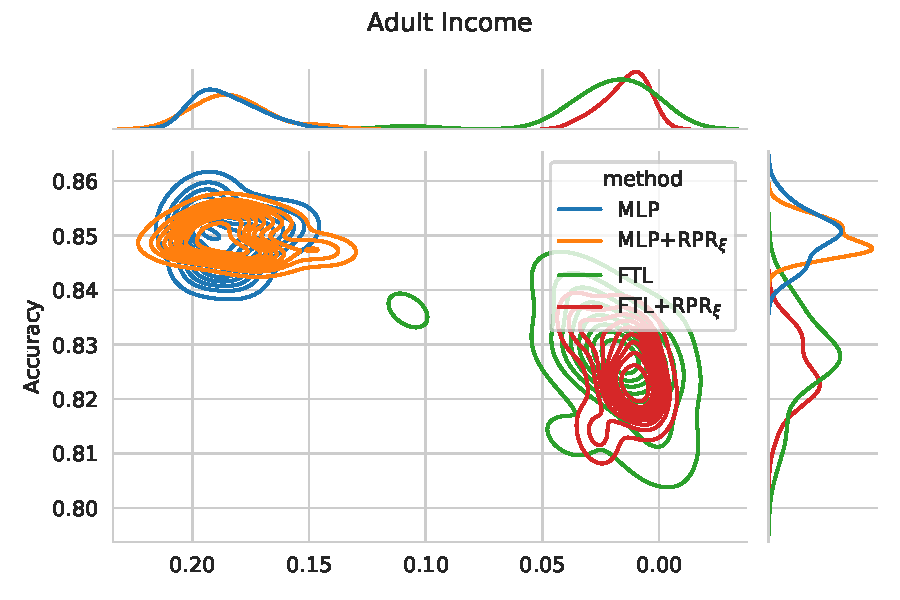
\includegraphics[width=1\linewidth]{images/pareto_acc_parity_adult_rpr.pdf}
\end{subfigure}
\begin{subfigure}{.45\linewidth}
    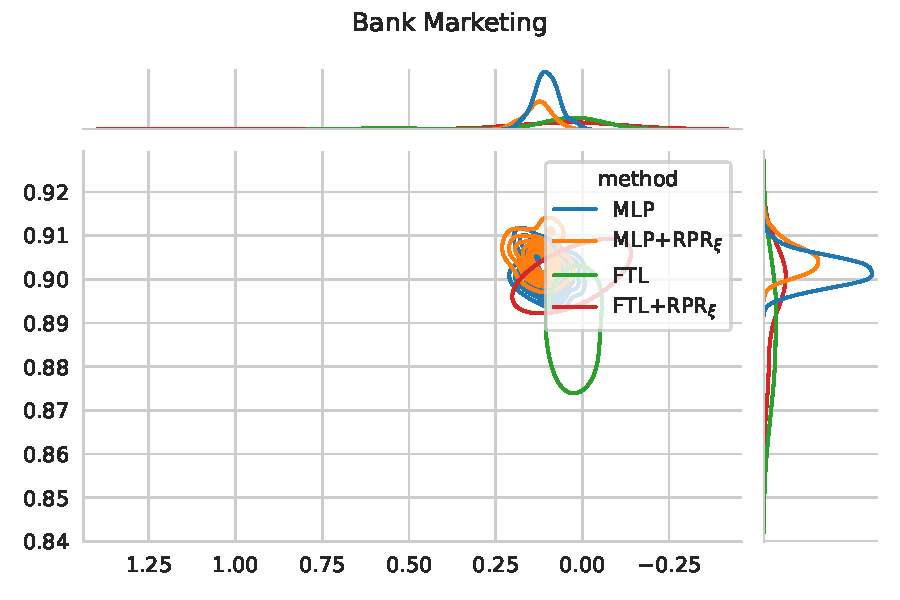
\includegraphics[width=1\linewidth]{images/pareto_acc_parity_bank_rpr.pdf}
\end{subfigure}

\begin{subfigure}{.45\linewidth}
    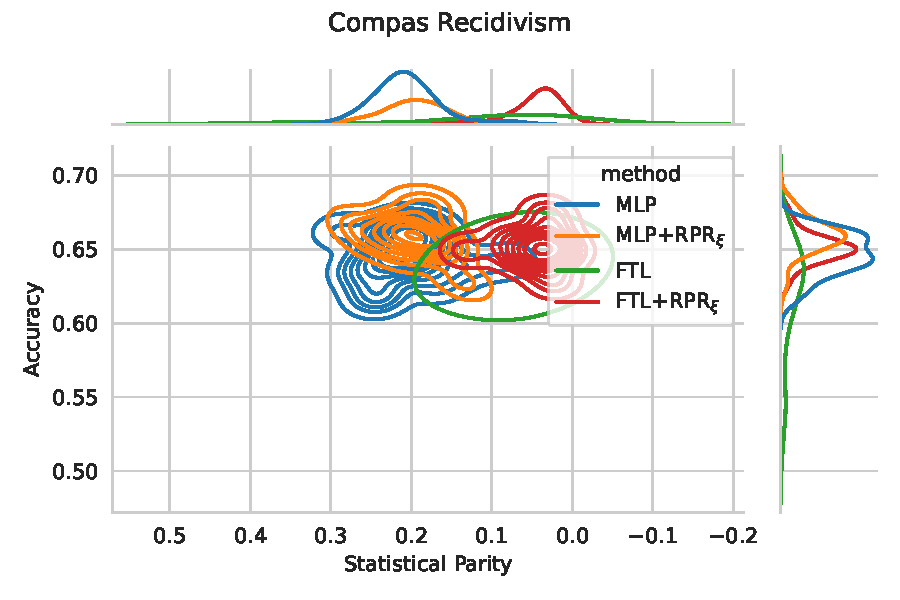
\includegraphics[width=1\linewidth]{images/pareto_acc_parity_compas_rpr.pdf}
\end{subfigure}
\begin{subfigure}{.45\linewidth}
    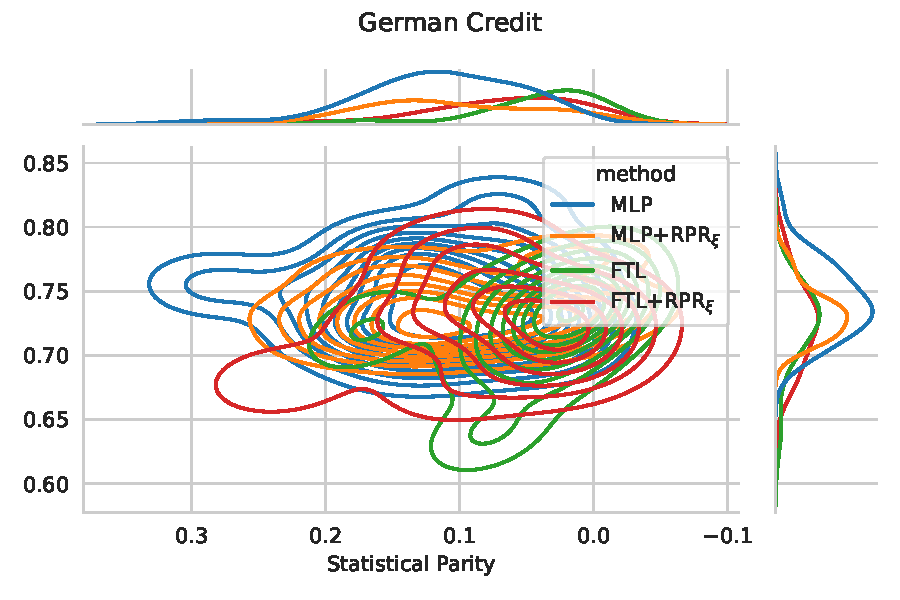
\includegraphics[width=1\linewidth]{images/pareto_acc_parity_german_rpr.pdf}
\end{subfigure}
\end{figure}

\begin{table}
    \centering
    \caption{Mean and standard deviation metric values optimizing Accuracy and Equal Opportunity in comparison with Redlining Penalty Regularizer.}\label{tab:complete_acc_opportunity_rpr}
    {\tiny \begin{tabular}{llrrr}
    \toprule
    Dataset & Method & $\uparrow\;$Fitness & $\uparrow\;$Accuracy & $\downarrow\;$Eq. Opp. \\
    \midrule
        
    \multirow{8}{*}{\shortstack[l]{Adult\\ Income}} & FTL & $0.812 \; (\pm0.03)$ & $0.845 \; (\pm0.01)$ & $0.034 \; (\pm0.02)$ \\
     & FTL+RPR$_{\xi}$ & $\textbf{0.815} \; (\pm0.02)$ & $0.847 \; (\pm0.00)$ & $\textbf{0.031} \; (\pm0.02)$ \\
     & MLP & $0.758 \; (\pm0.04)$ & $0.848 \; (\pm0.00)$ & $0.090 \; (\pm0.04)$ \\
     & MLP+L2 & $0.750 \; (\pm0.04)$ & $\textbf{0.850} \; (\pm0.00)$ & $0.100 \; (\pm0.04)$ \\
     & MLP+RPR$_{\rho_s}$ & $0.748 \; (\pm0.03)$ & $0.849 \; (\pm0.00)$ & $0.101 \; (\pm0.03)$ \\
     & MLP+RPR$_{\rho}$ & $0.750 \; (\pm0.04)$ & $0.848 \; (\pm0.00)$ & $0.098 \; (\pm0.04)$ \\
     & MLP+RPR$_{\tau}$ & $0.751 \; (\pm0.03)$ & $0.849 \; (\pm0.00)$ & $0.098 \; (\pm0.03)$ \\
     & MLP+RPR$_{\xi}$ & $0.757 \; (\pm0.05)$ & $0.849 \; (\pm0.00)$ & $0.091 \; (\pm0.05)$ \\
    \midrule
    \multirow{8}{*}{\shortstack[l]{Bank\\ Marketing}} & FTL & $0.781 \; (\pm0.17)$ & $0.883 \; (\pm0.02)$ & $0.102 \; (\pm0.17)$ \\
     & FTL+RPR$_{\xi}$ & $0.802 \; (\pm0.08)$ & $0.892 \; (\pm0.01)$ & $0.090 \; (\pm0.09)$ \\
     & MLP & $0.803 \; (\pm0.07)$ & $0.902 \; (\pm0.00)$ & $0.099 \; (\pm0.07)$ \\
     & MLP+L2 & $0.791 \; (\pm0.08)$ & $\textbf{0.903} \; (\pm0.00)$ & $0.112 \; (\pm0.07)$ \\
     & MLP+RPR$_{\rho_s}$ & $0.824 \; (\pm0.06)$ & $0.902 \; (\pm0.00)$ & $0.078 \; (\pm0.06)$ \\
     & MLP+RPR$_{\rho}$ & $0.798 \; (\pm0.07)$ & $0.901 \; (\pm0.00)$ & $0.103 \; (\pm0.07)$ \\
     & MLP+RPR$_{\tau}$ & $0.822 \; (\pm0.07)$ & $0.901 \; (\pm0.00)$ & $0.079 \; (\pm0.07)$ \\
     & MLP+RPR$_{\xi}$ & $\textbf{0.839} \; (\pm0.05)$ & $\textbf{0.903} \; (\pm0.00)$ & $\textbf{0.063} \; (\pm0.04)$ \\
    \midrule
    \multirow{8}{*}{\shortstack[l]{COMPAS\\ Recidivism}} & FTL & $\textbf{0.614} \; (\pm0.03)$ & $0.645 \; (\pm0.03)$ & $\textbf{0.031} \; (\pm0.02)$ \\
     & FTL+RPR$_{\xi}$ & $0.598 \; (\pm0.03)$ & $0.639 \; (\pm0.02)$ & $0.041 \; (\pm0.03)$ \\
     & MLP & $0.498 \; (\pm0.04)$ & $0.646 \; (\pm0.01)$ & $0.148 \; (\pm0.04)$ \\
     & MLP+L2 & $0.519 \; (\pm0.04)$ & $0.647 \; (\pm0.02)$ & $0.128 \; (\pm0.03)$ \\
     & MLP+RPR$_{\rho_s}$ & $0.520 \; (\pm0.03)$ & $0.651 \; (\pm0.01)$ & $0.131 \; (\pm0.03)$ \\
     & MLP+RPR$_{\rho}$ & $0.503 \; (\pm0.06)$ & $0.649 \; (\pm0.01)$ & $0.146 \; (\pm0.05)$ \\
     & MLP+RPR$_{\tau}$ & $0.506 \; (\pm0.04)$ & $0.647 \; (\pm0.01)$ & $0.141 \; (\pm0.04)$ \\
     & MLP+RPR$_{\xi}$ & $0.536 \; (\pm0.03)$ & $\textbf{0.663} \; (\pm0.01)$ & $0.127 \; (\pm0.03)$ \\
    \midrule
    \multirow{8}{*}{\shortstack[l]{German\\ Credit}} & FTL & $0.676 \; (\pm0.06)$ & $\textbf{0.751} \; (\pm0.02)$ & $0.075 \; (\pm0.06)$ \\
     & FTL+RPR$_{\xi}$ & $0.665 \; (\pm0.06)$ & $0.736 \; (\pm0.03)$ & $0.071 \; (\pm0.05)$ \\
     & MLP & $0.673 \; (\pm0.06)$ & $0.739 \; (\pm0.03)$ & $0.066 \; (\pm0.05)$ \\
     & MLP+L2 & $0.652 \; (\pm0.04)$ & $0.736 \; (\pm0.03)$ & $0.084 \; (\pm0.05)$ \\
     & MLP+RPR$_{\rho_s}$ & $0.667 \; (\pm0.06)$ & $0.739 \; (\pm0.03)$ & $0.072 \; (\pm0.05)$ \\
     & MLP+RPR$_{\rho}$ & $0.687 \; (\pm0.04)$ & $0.749 \; (\pm0.04)$ & $0.062 \; (\pm0.03)$ \\
     & MLP+RPR$_{\tau}$ & $\textbf{0.702} \; (\pm0.04)$ & $0.736 \; (\pm0.02)$ & $\textbf{0.034} \; (\pm0.03)$ \\
     & MLP+RPR$_{\xi}$ & $\textbf{0.702} \; (\pm0.05)$ & $0.750 \; (\pm0.02)$ & $0.048 \; (\pm0.04)$ \\
     \bottomrule
\end{tabular} }
\end{table}

\begin{figure}
\centering
\caption{Metric distribution optimizing Acc. and Equal Opportunity in comparison with Redlining Penalty Regularization across multiple resample runs. Corresponding values available at Table~\ref{tab:complete_acc_opportunity_rpr}.}
\label{fig:complete_mcc_apportunity_rpr}
\begin{subfigure}{.45\linewidth}
    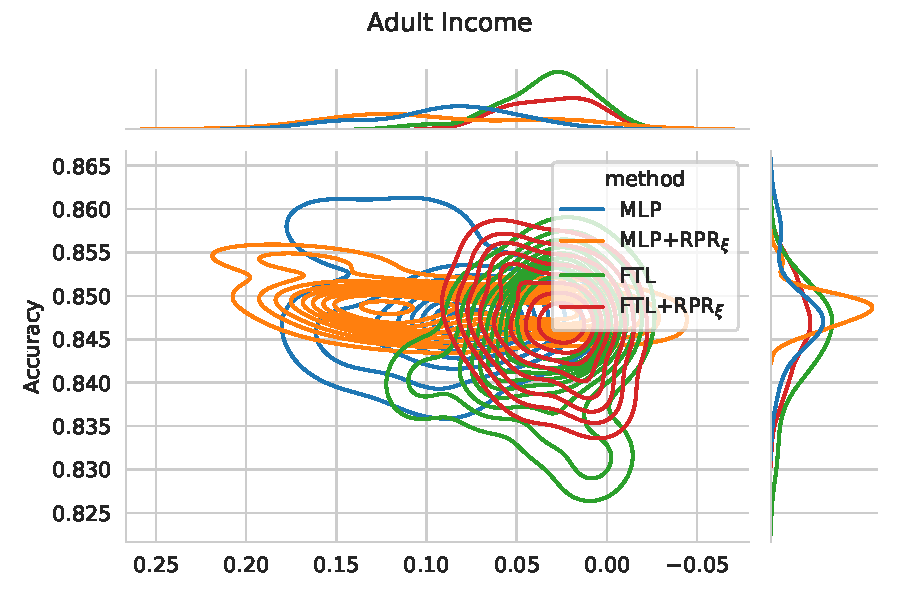
\includegraphics[width=1\linewidth]{images/pareto_acc_opportunity_adult_rpr.pdf}
\end{subfigure}
\begin{subfigure}{.45\linewidth}
    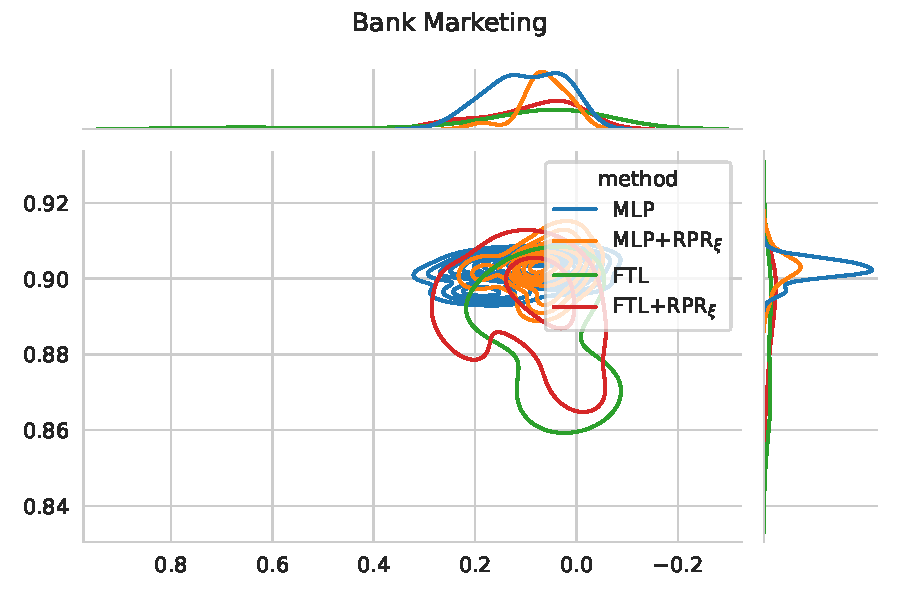
\includegraphics[width=1\linewidth]{images/pareto_acc_opportunity_bank_rpr.pdf}
\end{subfigure}

\begin{subfigure}{.45\linewidth}
    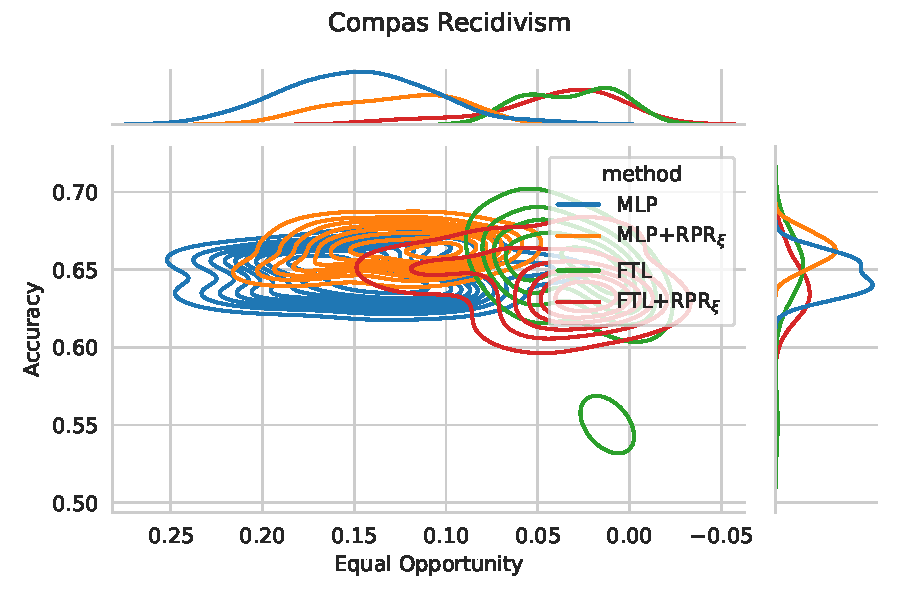
\includegraphics[width=1\linewidth]{images/pareto_acc_opportunity_compas_rpr.pdf}
\end{subfigure}
\begin{subfigure}{.45\linewidth}
    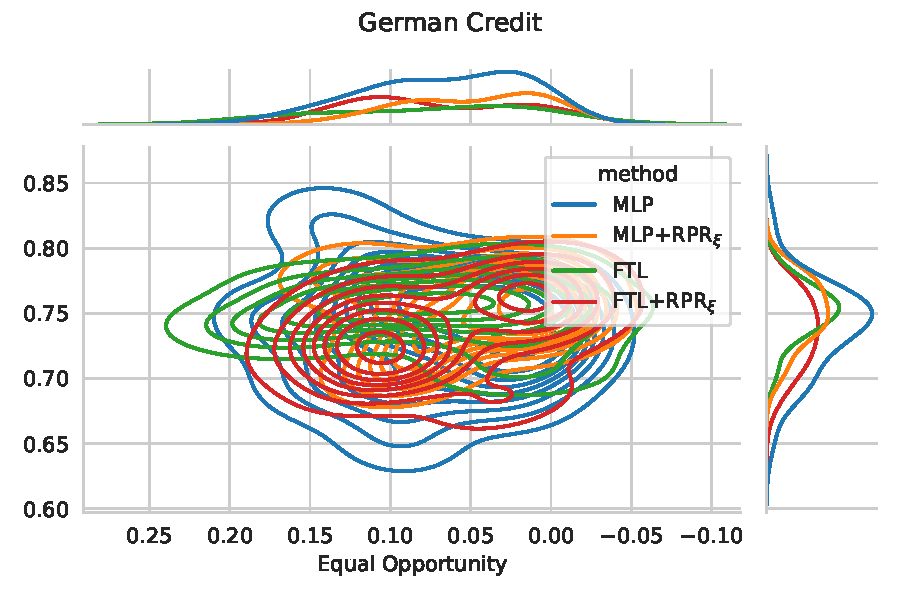
\includegraphics[width=1\linewidth]{images/pareto_acc_opportunity_german_rpr.pdf}
\end{subfigure}
\end{figure}

 \begin{table}
    \centering
    \caption{Mean and standard deviation metric values optimizing Accuracy and Equalized Odds in comparison with Redlining Penalty Regularizer.}\label{tab:complete_acc_odds_rpr}
    {\tiny \begin{tabular}{llrrr}
    \toprule
    Dataset & Method & $\uparrow\;$Fitness & $\uparrow\;$Accuracy & $\downarrow\;$Eq. Odds \\
    \midrule
        
    \multirow{8}{*}{\shortstack[l]{Adult\\ Income}} & FTL & $0.798 \; (\pm0.02)$ & $0.841 \; (\pm0.01)$ & $0.043 \; (\pm0.02)$ \\
     & FTL+RPR$_{\xi}$ & $\textbf{0.805} \; (\pm0.02)$ & $0.843 \; (\pm0.01)$ & $\textbf{0.038} \; (\pm0.02)$ \\
     & MLP & $0.760 \; (\pm0.02)$ & $\textbf{0.849} \; (\pm0.00)$ & $0.089 \; (\pm0.02)$ \\
     & MLP+L2 & $0.762 \; (\pm0.02)$ & $\textbf{0.849} \; (\pm0.00)$ & $0.086 \; (\pm0.02)$ \\
     & MLP+RPR$_{\rho_s}$ & $0.772 \; (\pm0.02)$ & $\textbf{0.849} \; (\pm0.00)$ & $0.076 \; (\pm0.02)$ \\
     & MLP+RPR$_{\rho}$ & $0.759 \; (\pm0.02)$ & $\textbf{0.849} \; (\pm0.00)$ & $0.090 \; (\pm0.02)$ \\
     & MLP+RPR$_{\tau}$ & $0.753 \; (\pm0.03)$ & $\textbf{0.849} \; (\pm0.00)$ & $0.096 \; (\pm0.02)$ \\
     & MLP+RPR$_{\xi}$ & $0.772 \; (\pm0.02)$ & $\textbf{0.849} \; (\pm0.00)$ & $0.077 \; (\pm0.02)$ \\
    \midrule
    \multirow{8}{*}{\shortstack[l]{Bank\\ Marketing}} & FTL & $\textbf{0.846} \; (\pm0.03)$ & $0.890 \; (\pm0.01)$ & $\textbf{0.044} \; (\pm0.04)$ \\
     & FTL+RPR$_{\xi}$ & $0.831 \; (\pm0.05)$ & $0.892 \; (\pm0.01)$ & $0.061 \; (\pm0.05)$ \\
     & MLP & $0.845 \; (\pm0.03)$ & $0.901 \; (\pm0.00)$ & $0.057 \; (\pm0.03)$ \\
     & MLP+L2 & $0.821 \; (\pm0.04)$ & $\textbf{0.903} \; (\pm0.00)$ & $0.082 \; (\pm0.04)$ \\
     & MLP+RPR$_{\rho_s}$ & $0.838 \; (\pm0.04)$ & $\textbf{0.903} \; (\pm0.00)$ & $0.065 \; (\pm0.04)$ \\
     & MLP+RPR$_{\rho}$ & $0.828 \; (\pm0.05)$ & $0.902 \; (\pm0.00)$ & $0.073 \; (\pm0.05)$ \\
     & MLP+RPR$_{\tau}$ & $0.822 \; (\pm0.04)$ & $0.902 \; (\pm0.00)$ & $0.079 \; (\pm0.04)$ \\
     & MLP+RPR$_{\xi}$ & $0.830 \; (\pm0.03)$ & $0.902 \; (\pm0.00)$ & $0.072 \; (\pm0.03)$ \\
    \midrule
    \multirow{8}{*}{\shortstack[l]{COMPAS\\ Recidivism}} & FTL & $0.545 \; (\pm0.10)$ & $0.631 \; (\pm0.05)$ & $0.086 \; (\pm0.08)$ \\
     & FTL+RPR$_{\xi}$ & $\textbf{0.594} \; (\pm0.04)$ & $0.647 \; (\pm0.02)$ & $\textbf{0.053} \; (\pm0.04)$ \\
     & MLP & $0.449 \; (\pm0.04)$ & $0.649 \; (\pm0.01)$ & $0.200 \; (\pm0.03)$ \\
     & MLP+L2 & $0.452 \; (\pm0.04)$ & $0.649 \; (\pm0.01)$ & $0.197 \; (\pm0.04)$ \\
     & MLP+RPR$_{\rho_s}$ & $0.464 \; (\pm0.03)$ & $0.650 \; (\pm0.01)$ & $0.186 \; (\pm0.03)$ \\
     & MLP+RPR$_{\rho}$ & $0.449 \; (\pm0.05)$ & $0.650 \; (\pm0.01)$ & $0.201 \; (\pm0.04)$ \\
     & MLP+RPR$_{\tau}$ & $0.463 \; (\pm0.05)$ & $0.650 \; (\pm0.01)$ & $0.187 \; (\pm0.05)$ \\
     & MLP+RPR$_{\xi}$ & $0.497 \; (\pm0.04)$ & $\textbf{0.667} \; (\pm0.01)$ & $0.170 \; (\pm0.03)$ \\
    \midrule
    \multirow{8}{*}{\shortstack[l]{German\\ Credit}} & FTL & $0.669 \; (\pm0.05)$ & $0.712 \; (\pm0.02)$ & $\textbf{0.043} \; (\pm0.07)$ \\
     & FTL+RPR$_{\xi}$ & $0.631 \; (\pm0.06)$ & $0.721 \; (\pm0.03)$ & $0.090 \; (\pm0.08)$ \\
     & MLP & $0.619 \; (\pm0.07)$ & $0.740 \; (\pm0.03)$ & $0.121 \; (\pm0.07)$ \\
     & MLP+L2 & $\textbf{0.675} \; (\pm0.05)$ & $\textbf{0.750} \; (\pm0.02)$ & $0.075 \; (\pm0.04)$ \\
     & MLP+RPR$_{\rho_s}$ & $0.647 \; (\pm0.06)$ & $0.742 \; (\pm0.03)$ & $0.096 \; (\pm0.05)$ \\
     & MLP+RPR$_{\rho}$ & $0.641 \; (\pm0.04)$ & $0.734 \; (\pm0.03)$ & $0.093 \; (\pm0.04)$ \\
     & MLP+RPR$_{\tau}$ & $0.647 \; (\pm0.07)$ & $0.748 \; (\pm0.03)$ & $0.101 \; (\pm0.07)$ \\
     & MLP+RPR$_{\xi}$ & $0.640 \; (\pm0.06)$ & $0.748 \; (\pm0.02)$ & $0.107 \; (\pm0.06)$ \\
     \bottomrule
\end{tabular}}
\end{table}

\begin{figure}
\centering
\caption{Metric distribution optimizing Acc. and Equalized Odds in comparison with Redlining Penalty Regularization across multiple resample runs. Corresponding values available at Table~\ref{tab:complete_acc_odds_rpr}.}
\label{fig:complete_acc_odds_rpr}
\begin{subfigure}{.45\linewidth}
    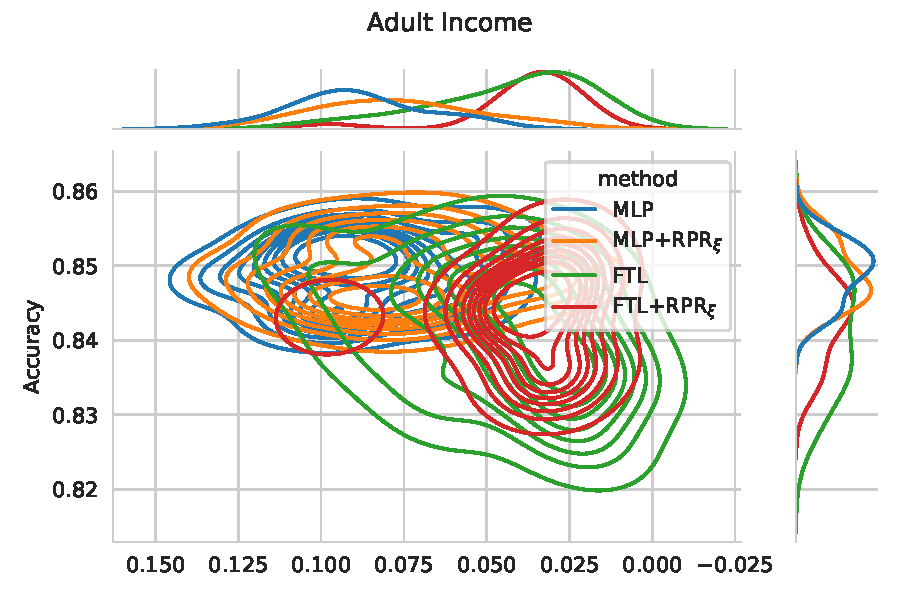
\includegraphics[width=1\linewidth]{images/pareto_acc_odds_adult_rpr.pdf}
\end{subfigure}
\begin{subfigure}{.45\linewidth}
    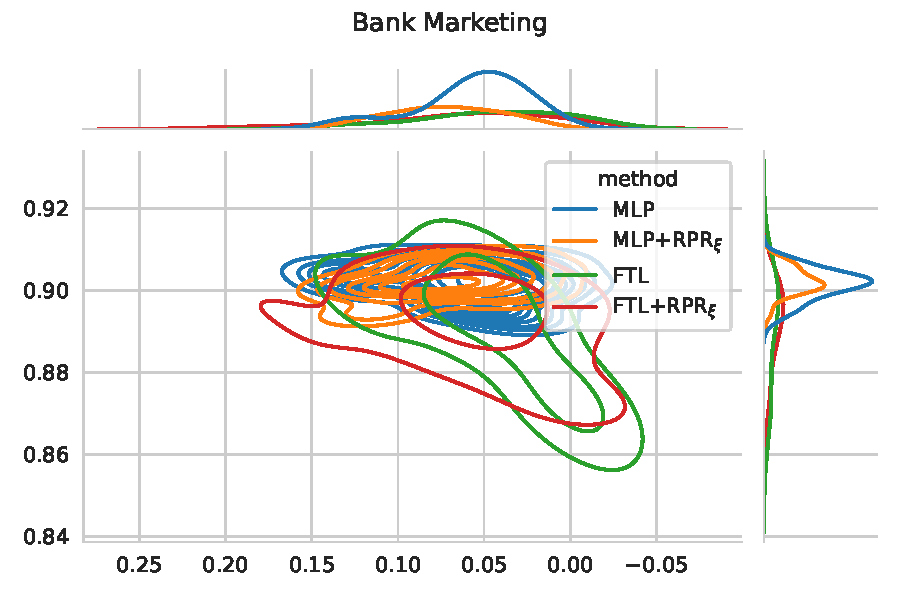
\includegraphics[width=1\linewidth]{images/pareto_acc_odds_bank_rpr.pdf}
\end{subfigure}

\begin{subfigure}{.45\linewidth}
    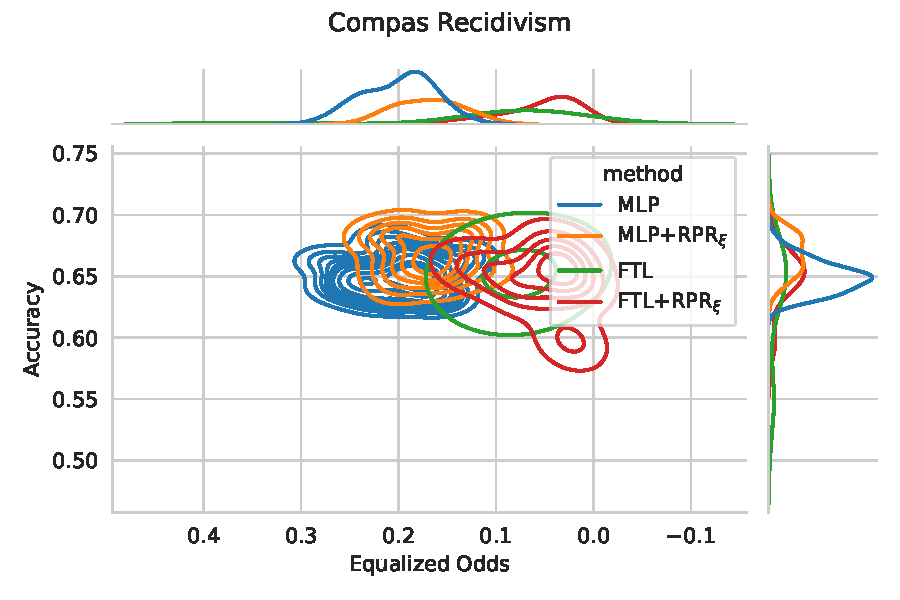
\includegraphics[width=1\linewidth]{images/pareto_acc_odds_compas_rpr.pdf}
\end{subfigure}
\begin{subfigure}{.45\linewidth}
    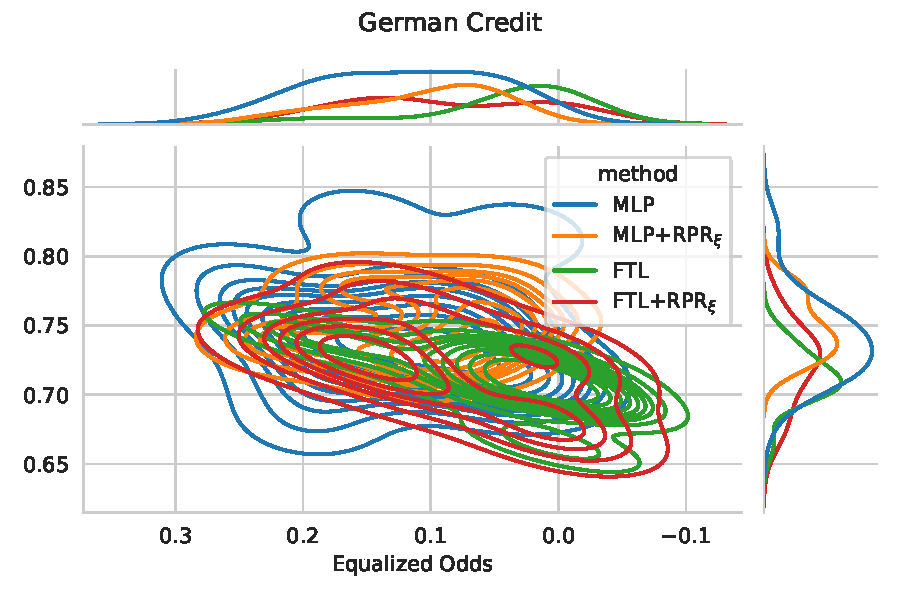
\includegraphics[width=1\linewidth]{images/pareto_acc_odds_german_rpr.pdf}
\end{subfigure}
\end{figure}
